\documentclass[11pt]{article}
\usepackage[a4paper, total={6in, 8in}]{geometry}
\usepackage{amsmath}
\usepackage{amsthm}
\usepackage{graphicx}
\usepackage{amsfonts}
\usepackage{xcolor}
\usepackage{enumerate}
\usepackage[hidelinks]{hyperref}
\pagenumbering{roman}
\begin{document}

\newtheorem{theorem}{Theorem}
\numberwithin{theorem}{section}
\theoremstyle{definition}
\newtheorem{definition}{Definition}
\newtheorem{proposition}{Proposition}
\newtheorem{example}{Example}
\newtheorem{lemma}{Lemma}
\newtheorem{corollary}{Corollary}
\numberwithin{definition}{section}
\numberwithin{proposition}{section}
\numberwithin{example}{section}
\numberwithin{lemma}{section}
\numberwithin{corollary}{section}
\newcommand{\uw}{\mathcal{U}(W,X)}
\newcommand{\W}{$(W,S)$}
\newcommand{\ix}{\textit}
\newcommand{\tr}{\textcolor{red}}
\newcommand{\sg}{$\Sigma$}


\title{Shadows in Coxeter complexes}
\author{Megan Masters}
\maketitle



\begin{abstract}
    


In this project, we will be looking at Tits buildings, and in particular Coxeter complexes. We look at buildings as geometric objects, combinatorial objects, and as representations of groups. These viewpoints give us unique information about the building and its group of automorphisms. We will look at galleries in buildings, which are sequences of alcoves of a building. We then look at foldings of these galleries in Coxeter complexes, with respect to an orientation. An important combinatorial question of foldings is which alcoves of the Coxeter complex can be reached by folding a certain gallery. We call this set the \ix{shadow} of a gallery. We shall see some progress in answering the question of calculating the shadow, and we will discuss tools which could be used to improve these answers. 

\end{abstract}
\begin{center}
    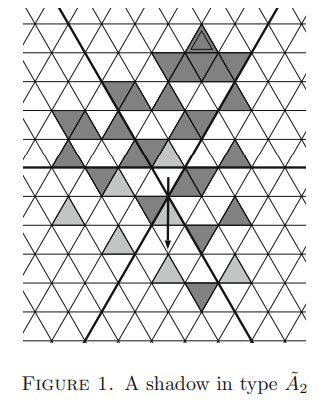
\includegraphics[scale=1.5]{Screenshot 2023-03-28 114049.png}\\
\end{center}
\newpage
\tableofcontents
\newpage
\pagenumbering{arabic}
\section{Introduction}
Buildings were first defined by Jacques Tits in the 1950s \cite{TITS}. They are geometric objects which were first created to help us describe algebraic simple groups and semi-simple Lie groups. In this project, we will be studying Coxeter complexes, which are examples of buildings. They also give us a tool to help us to form more complicated buildings. We will mostly restrict our discussion to affine Coxeter complexes and their finite quotients.

We ultimately want to look at walks, which we call galleries, around the alcoves of Coxeter complexes. In this paper, we focus on alcove to alcove orientations. Other papers, including Schwer \cite{WILD}, also discuss galleries which start and end at vertices. These galleries, and their positive foldings, are used in a wide range of mathematics. Positive foldings of galleries were first introduced in 2005 by Gaussent and Littelmann \cite{LSGAL}. They can be used to compute Hall-Littlewood polynomials \cite{HL}, and have been used to study MV polytopes \cite{MVPOLY}. There is also a link between folded galleries and affine Deligne-Lusztig varieties \cite{DEL}. We define the shadow of a gallery as the set of end alcoves which can be reached by a positive folding of the gallery. For a more in depth discussion on the applications of shadows, Schwer has written a detailed paper \cite{WILD}.

!!! In this paper, we restrict to considering shadows of galleries which are retractions based at alcoves or at a chamber at infinity. There is further research \cite{NAQVI} which considers retractions and the respective shadows with respect to chimney orientations.

 

Our main example arises from the Coxeter group $\tilde{A}_2$. This has presentation
\[\tilde{A}_2=\langle s_0,s_1,s_2\mid s_i^2=1, (s_0s_1)^3=(s_0s_2)^3=(s_1s_2)^3=1\rangle.\]
The Coxeter complex associated with this Coxeter system is the tiling of the plane by equilateral triangles. 

\begin{center}
    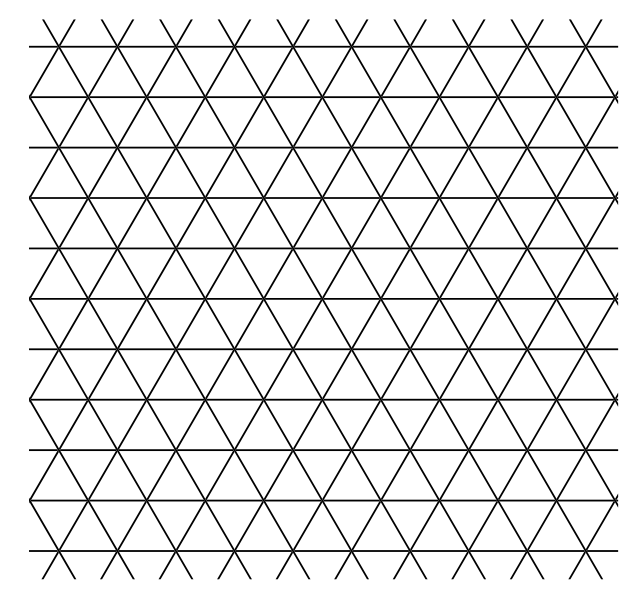
\includegraphics[scale=0.4]{Screenshot 2023-03-28 114008.png}\\
\end{center}

Throughout the paper, we will use this Coxeter complex to illustrate definitions and concepts. We will also explore the finite Coxeter group $A_2$, which is a quotient of $\tilde{A}_2$. 
%We have a finite Coxeter group within this group
% \[A_2=\langle s_1,s_2\mid s_i^2=1, (s_1s_2)^3=1\rangle.\]
% Within the Coxeter complex, this finite Coxeter group is represented by hexagons. The elements $s_1$ and $s_2$ act on the triangles in these hexagons, with each line in the picture acting as a reflection. 

% \begin{center}
%     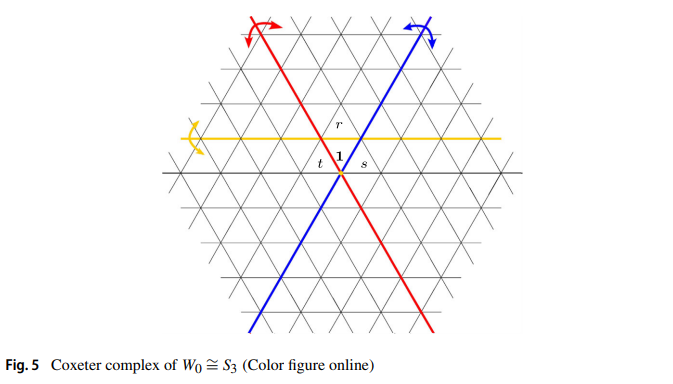
\includegraphics[scale=0.7]{Screenshot 2023-03-14 150033.png}\\
% \end{center}

% We call this finite Coxeter complex the boundary of the infinite Coxeter complex. We can represent the boundary as a tiling of an $(n-1)$-sphere, where $n$ is the dimension of the tiled space of the infinite Coxeter complex. So in this case, we can represent the boundary as a tiling of $S^1$.

% \begin{center}
%     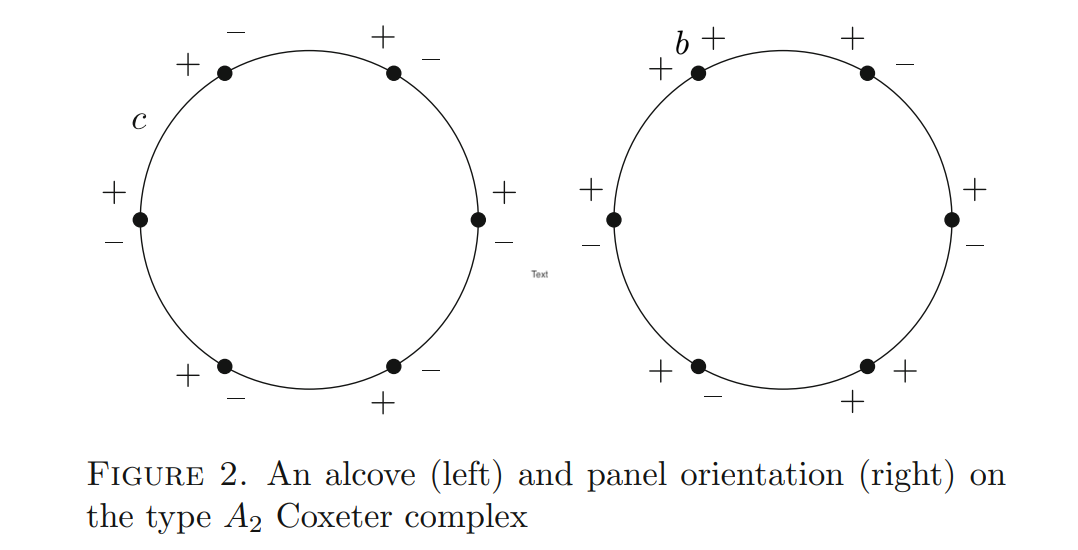
\includegraphics[scale=0.6]{Screenshot 2023-02-03 102201.png}\\
% \end{center}

% Then if we fix any centre of a hexagon in the infinite Coxeter complex, we have \ix{Weyl chambers} which are the infinite wedges pointing out in the direction of the boundary. Then there is an obvious projection with a triangle of the infinite complex being sent to the element of the boundary which is associated to the Weyl chamber containing the triangle.



In \hyperref[2]{Section 2}, we define a general chamber system, and give a few important examples of chamber systems. We will then, in \hyperref[3]{Section 3}, look at specific examples of chamber systems called Coxeter complexes. These arise from Coxeter groups. Next, we will look at galleries of Coxeter complexes, which are walks around the alcoves. Then, in \hyperref[4]{Section 4}, we will define a building and see how we can construct buildings from Coxeter complexes. We will discuss two different retractions of a building onto one of its Coxeter complexes in \hyperref[5]{Section 5}. In \hyperref[6]{Section 6}, we define orientations of Coxeter complexes, specifically looking at the orientations with respect to some alcove and some chamber at infinity. Then \hyperref[7]{Section 7} covers folded galleries. These are galleries which have been partially reflected along walls of the Coxeter complex. In \hyperref[8]{Section 8}, we define shadows of galleries in Coxeter complexes, and look at the relationship between retractions and shadows. This relationship is our motivation for studying shadows. Finally, in \hyperref[9]{Section 9}, we will look at the progress which has been made so far in answering the question of calculating the shadows of galleries. 




\section{Chamber systems} \label{2}
We first start our exploration of buildings with an abstract chamber system - a set with some equivalence relations on it.  

\begin{definition}
    A set $C$ is called a \ix{chamber system} over a set $I$ if each $i\in I$ is an equivalence relation on the elements of $C$. Each $i$ partitions our set $C$ into equivalence classes. We say two elements $x,y\in C$ are \ix{i-adjacent}, and we write $x\sim_{i} y$, if they lie in the same part of the partition, i.e.\ they are equivalent with respect to the equivalence relation corresponding to $i$. The elements of $C$ are called \ix{chambers}. The \ix{rank} of a chamber system is the size of $I$. 
\end{definition}


A very important example is obtained by looking at a group $G$, and a subgroup $B$, and defining the following equivalence relations: 

\begin{example}\label{S3}
    Consider a group $G$, a subgroup $B$, and an indexing set $I$, such that there exists $B<P_i<G$ for all $i\in I$. Then we take our chamber system $C$ to be the left cosets of $B$, and we define an equivalence relation
    \[gB\sim_{i}hB \textnormal{ if and only if }gP_i=hP_i.\]

    For an explicit example, consider the group $G=S_3$, let $B=\{1\}$, and let $P_1=\langle (1,2)\rangle$, $P_2=\langle (2,3)\rangle$. Then our chambers are the elements of $G$, and two elements $g,h$ are $i$-adjacent if $g=h\cdot(i,i+1)$. 
\end{example}

We now look at galleries of a chamber system. These are walks around the chambers, where we only move from one chamber to an adjacent chamber. 

\begin{definition}\label{gallery}
    A finite sequence $(c_0,\hdots ,c_k)$ such that $c_i$ is adjacent to $c_{i+1}$ is called a \ix{gallery}. Its \ix{type} is a word $i_1\hdots i_k$ in $I$ such that  $c_{j-1}$ is $i_j$-adjacent to $c_{j}$. 
\end{definition}

In Definition \ref{comb.gallery} we will define a combinatorial gallery, which is a gallery in the specific case that our chamber system is a Coxeter complex. A combinatorial gallery encodes the same information as the gallery defined above, but also encodes information about the geometric structure of the complex, in the form of panels. 

\begin{definition}\label{residue}
    We call a chamber system $C$ \ix{connected} if there is a gallery between any two chambers. Given a subset $J\subset I$, a \ix{residue of type J} is a $J$-connected component, i.e.\ there is a gallery between any two elements of a $J$-connected component whose type is a word in $J$. The \ix{cotype} of $J$ is $I-J$. The corank of $J$ is $\mid I\mid -\mid J\mid $, i.e.\ the size of the cotype of $J$. 
\end{definition}
% \begin{definition}
%     Let $R$ be a $J$-residue and $S$ be a $K$-residue. Then $S$ is a \ix{face} of $R$ if $R\subset S$ and $J\subset K$. 
% \end{definition}

% Observe that if $R$ is a residue of cotype $J$, we have:
% \begin{enumerate}
%     \item for $K\subset J$, there is a unique face of $R$ which has cotype $K$.
%     \item Let $S_1,S_2$ be faces of $R$ with cotypes $K_1$ and $K_2$. Then $S_1$ and $S_2$ have a shared face of cotype $K_1\cap K_2$. 
% \end{enumerate}


% \subsection{The geometric realisation}

% \tr{This section needs quite a bit of rewording.}

% We now want to construct a geometric realisation of this chamber system. We construct a simplicial complex, where each simplex represents a residue of our chamber system.

% \begin{definition}
%     Let $R$ be a $J$-residue and $S$ be a $K$-residue. Then $S$ is a \ix{face} of $R$ if $R\subset S$ and $J\subset K$. 
% \end{definition}

% Observe that if $R$ is a residue of cotype $J$, we have
% \begin{enumerate}
%     \item for $K\subset J$, there is a unique face of $R$ which has cotype $K$.
%     \item Let $S_1,S_2$ be faces of $R$ with cotypes $K_1$ and $K_2$. Then $S_1$ and $S_2$ have a shared face of cotype $K_1\cap K_2$. 
% \end{enumerate}


% With these observations, we can form a \ix{cell complex} of our chamber system. To do this, we form a vertex for each residue of corank 1. Then, we can associate to each residue of cotype $\{i,j\}$ an edge. From the observation above, this has, as its boundary, the residues of cotype $\{i\}$ and of cotype $\{j\}$. 

% Then this can be continued inductively. So given a residue $R$ which has cotype of size $r$, we associate a dimension $r-1$ simplex. Now the faces of this simplex are exactly the faces of $R$, as defined above. 

% \begin{example}
%     Consider our specific example of the group $S_3$ from example \ref{S3}. As $I=\{1,2\}$, our corank 1 residues are equal to our rank 1 residues. Here, our rank 1 residues are pairs of elements $g,h$ satisfying $g=h\cdot (i,i+1)$. 
% \end{example}

% \begin{center}
%     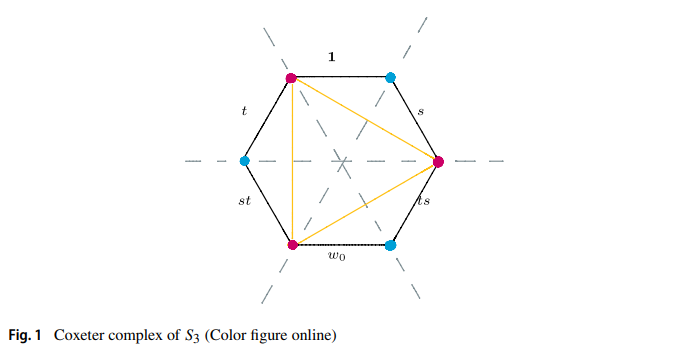
\includegraphics[scale=0.8]{Screenshot 2023-03-20 113453.png}
% \end{center}

\subsection{$A_n(k)$ Buildings}

A key example of a chamber system is formed by considering the subspaces of an $n+1$ dimensional vector space $V$ over a field $k$. We define the chambers of our chamber system to be the maximal chains \[V_1\subset V_2\subset \hdots \subset V_n\] of subspaces of $V$, where $V_i$ has dimension $i$. We can then define adjacency by saying that two chains $V_1\subset V_2\subset \hdots \subset V_n$ and $V_1'\subset V_2'\subset \hdots \subset V_n'$ are $i$-adjacent if $V_j=V_j'$ for all $j\neq i$. Then the residues of type $i$ correspond to 1-spaces in the 2-space $V_{i+1}/V_{i-1}$. 

% We then get a geometric realisation of this chamber system. Here, a residue of cotype $J=\{j_1,\hdots ,j_r\}$ corresponds to a sequence \[V_{j_1}\subset V_{j_2}\subset \hdots \subset V_{j_r}.\] This residue has chambers which are maximal flags $V_1'\subset V_2'\subset \hdots \subset V_n'$ such that $V_j'=V_j$ if $j\in J$. 

% In particular, residues of cotype $\{i\}$ correspond to the subspaces of $V$. 



\begin{center}
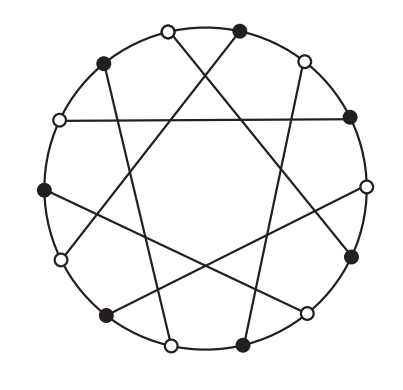
\includegraphics[scale=0.5]{Screenshot 2023-03-16 131651.png}
%\caption{The geometric representation of the chamber system $A_2(\mathbb{F}_2)$. Figure taken from \cite[p.2]{EVERITT}.}
\end{center}


\begin{example} \label{AnK}
    Here we have the geometric realisation of $A_2(\mathbb{F}_2)$. There are 7 one-dimensional subspaces, represented here as white, and there are 7 two-dimensional subspaces, represented as black. Here, the one-dimensional subspaces are
    \[\langle (1,0,0)\rangle, \langle (0,1,0)\rangle,\langle (0,0,1)\rangle,\langle (1,1,0)\rangle,\langle (1,0,1)\rangle,\langle (0,1,1)\rangle,\langle (1,1,1)\rangle.\]
    The two-dimensional subspaces are formed by taking the union of any two one-dimensional subspaces, or equivalently quotienting the whole vector space by one of the one-dimensional subspaces. 

    We have constructed this geometric realisation by associating each corank 1 residue, which correspond to the subspaces, to a point. Then the corank 2 residues, which are the chains of subspaces of length 2, are represented as line segments. Their endpoints are the 1-dimensional and 2-dimensional subspaces which create the chain. Therefore, white dots are connected to black dots.
\end{example}

\section{Coxeter complexes} \label{3}

We will now consider a class of chamber systems which are formed by considering a type of group called a Coxeter group. The corresponding chamber system is known as a \ix{Coxeter complex}. These objects have nice geometric realisations. In particular, the affine Coxeter groups create tilings of the Euclidean plane. Their finite quotients also appear in their geometric realisation. 

\begin{definition}
    A \ix{Coxeter group} is a group with presentation
    \[W=\langle s_1,\hdots , s_n \mid (s_is_j)^{m_{ij}}=1\rangle,\]
    where $m_{ii}=1$ for all $i$ and $m_{ij}\in \mathbb{Z}_{\geq 2}\cup\{\infty\}$ for all $i\neq j$. 
    A \ix{Coxeter system} is a pair $(W,S)$, where $W$ is a Coxeter group and $S$ is a set of generators of $W$ such that $W$ can be represented as above, with $S=\{s_1,\hdots,s_n\}$. The corresponding Coxeter matrix is the $n\times n$ matrix $(m_{ij})$. 
\end{definition}

!!! In this paper, we will restrict to Coxeter groups which are indecomposable, and so we are only considering Coxeter systems whose associated Coxeter diagram is connected. 

\begin{definition}
    If $f=i_1i_2\hdots  i_k$ is a word in $\{1,\hdots ,n\}$, we define $s_f$ as the element $s_{i_1}\hdots  s_{i_k}$ of $W$.
\end{definition}

A \ix{finite Coxeter group} is precisely a Coxeter group which has a finite number of elements. An \ix{affine Coxeter group} is a Coxeter group which has a normal abelian subgroup such that the quotient is finite. For instance, the finite group $A_2$ has presentation
\[A_2=\langle s_1,s_2\mid s_i^2=1, (s_1s_2)^3=1\rangle.\]
The corresponding affine Coxeter group is
\[\tilde{A}_2=\langle s_0,s_1,s_2\mid s_i^2=1, (s_0s_1)^3=(s_0s_2)^3=(s_1s_2)^3=1\rangle.\]
We can clearly see that quotienting $\tilde{A}_2$ by the normal abelian subgroup $\langle s_0\rangle$ gives us $A_2$. 


We can now construct a specific type of chamber system which arises from a Coxeter group. Given a Coxeter system $(W,S)$, take as chambers the elements of $W$, and define an $i$-adjacency by $w\sim_iws_i$, where $S=\{s_1,\hdots  ,s_n\}$ are the set of generators of the Coxeter group. If the Coxeter group has Coxeter matrix $M$, we call this building a \ix{Coxeter complex of type M}.


\subsection{The geometric realisation}
Now we can look at the geometric realisation of this chamber system. We will form a simplicial complex, where the simplicies represent the residues of our chamber system. 



\begin{definition}
    Let $(W,S)$ be a Coxeter system. Let $S'\subset S$. We define the \textit{standard parabolic subgroup} $W_{S'}$ of $W$ to be the subgroup generated by the subset $S'$. Then $(W_{S'},S')$ is also a Coxeter group. The \ix{parabolic sets} are the cosets of the standard parabolic subgroups. 
\end{definition}

This idea corresponds to our more general idea, from definition \ref{residues} of residues of chamber systems. For Coxeter complexes, we have an explicit definition of the residues as the parabolic sets. 

So first let us consider the rank 0 parabolic sets. This means that we have taken $S'=\emptyset$, and so our parabolic setss are of the form $xW_\emptyset=x\cdot{1}$. So our rank 0 parabolic sets are in bijection with the elements of $W$. Therefore, we form an $\mid I\mid -1$ dimensional simplex for each element of $W$. Now we force that two chambers are adjacent in our geometric realisation if and only if the two corresponding elements are adjacent in the chamber system. This exactly means that the corresponding elements $x,y$ of $W$ satisfy $x=y\cdot s_i$ for some $s_i\in S$. We call these simplicies \ix{chambers} if the group is finite, and \ix{alcoves} if the group is affine.

Now let us look at the codimension one simplicies. These are the \ix{panels} between each simplex defined above. These correspond to rank 1 parabolic sets, so subgroups of the form $xW_{\{s_i\}}$. This is exactly saying that the two chambers (or alcoves) lying on either side of the panel correspond to two elements of the Coxeter group which are $i$-adjacent. 


%The largest dimensional simplicies are formed 
%The zero dimensional simplicies of the geometric realisation of the Coxeter complex corresponds to the maximal parabolic subgroups. These maximal parabolic subgroups are formed by taking a subset of $S$ with one element removed. So these maximal parabolic subgroups are in bijection with the elements of $S$. 

%We can now form the 1 dimensional simplicies of our simplicial complex. For this, we take the parabolic subgroups which correspond to an element of the form $xW_{S\backslash \{s\}}$

% Here we formalise our definitions above:

% \begin{definition}
%     The maximal simplicies in the simplicial complex are called \textit{alcoves}, and the codimension-one faces are called \textit{panels}.  
% \end{definition}


%We note that there is a correspondence between between panels and vertices. This is because a vertex corresponds to an element of the form $xW_{S\backslash \{s\}}$, whilst a panel corresponds to an element of the form $xW_{S\backslash \{s\}}$. 

\begin{definition}
    If a panel $p$ corresponds to the element $xW_{\{s_i\}}$, we say that $p$ has \ix{type} $i$, and write $\tau(p)=i$. 
\end{definition}




Now we can look at the geometric realisation of $\tilde{A}_2$. Here our presentation is
 \[\tilde{A}_2=\langle s_0,s_1,s_2\mid s_i^2=1, (s_1s_2)^3=(s_2s_3)^3=(s_3s_1)^3=1\rangle.\]
To form our geometric realisation, we note that our indexing set is $I=\{0,1,2\}$. So we create a two dimension simplex for every element of $W$. So we have a triangle for each element of $W$. Then any two triangles are adjacent if their corresponding elements differ by multiplying by one element of $\{s_0,s_1,s_2\}$. 

\begin{center}
    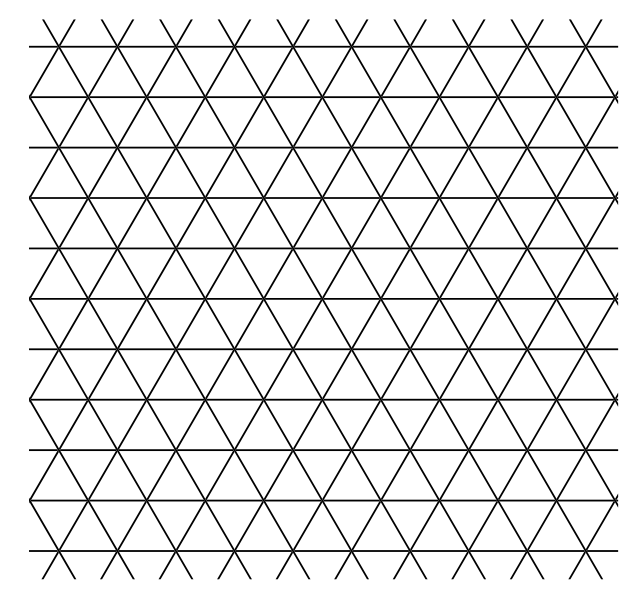
\includegraphics[scale=0.5]{Screenshot 2023-03-28 114008.png}\\
\end{center}

Now the triangles in this picture are the alcoves, and the edges between each triangle are the panels. Each panel has a type $i$, which is an element of the indexing set of $S$. This encodes that the two adjacent chambers to this panel are $i$-adjacent. 


Let us now form the geometric realisation of the group $A_2$. Here our presentation is 
\[A_2=\langle s_1,s_2\mid s_i^2=1, (s_1s_2)^3=1\rangle.\]
So our chamber system is the set of elements of $A_2$, with our indexing set $I=\{1,2\}$. Now for every element of $A_2$, we form a one-dimensional simplex, so a line segment. Then two line segments are connected by a point if their corresponding elements are adjacent. This means that we have six line segments, arranged in a circle. Each line segment is called a chamber (as $A_2$ is finite) and each point is a panel. Each panel is labelled with its type.

\begin{center}
    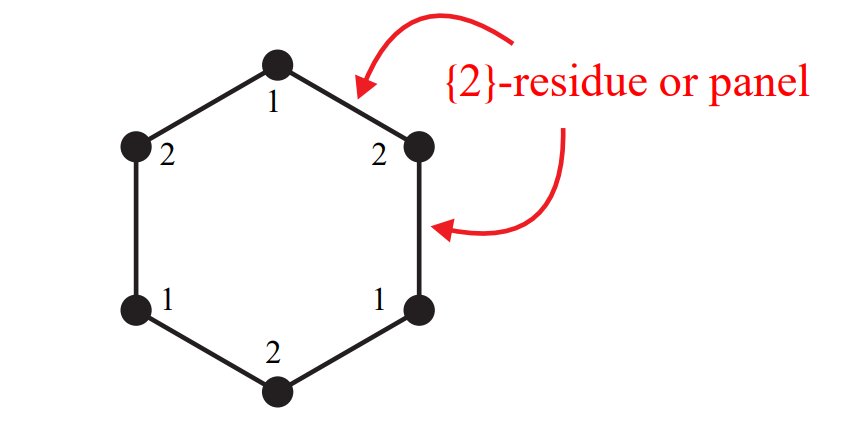
\includegraphics[scale=0.5]{Screenshot 2023-03-21 135437.png}\\
\end{center}

We can also see this structure hidden in the affine Coxeter complex of $\tilde{A}_2$. It is represented as the hexagons within the tiling of the plane. Then if we fix any centre of a hexagon in the infinite Coxeter complex, we have \ix{Weyl chambers} which are the infinite wedges pointing outwards. 

For a general affine Coxeter complex, we call the finite Coxeter complex the \ix{boundary} $\partial\Sigma$ of the infinite Coxeter complex $\Sigma$. We can represent the boundary as a tiling of an $(n-1)$-sphere, where $n$ is the dimension of the tiled space of the infinite Coxeter complex. 
%So in this case, we can represent the boundary as a tiling of $S^1$. 
%Then there is an obvious projection with a triangle of the infinite complex being sent to the element of the boundary which is associated to the Weyl chamber containing the triangle.




% \begin{center}
%     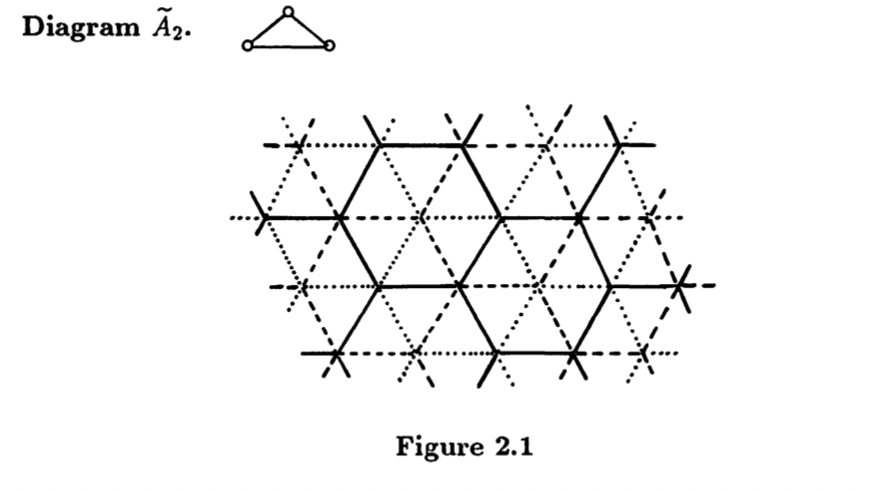
\includegraphics[scale=0.6]{Screenshot 2023-02-20 at 14.12.15.1.png}\\
% \end{center}



% Let us look at any hexagon within this picture. We note that any hexagon represents the finite group $A_2$ within the group $\tilde{A}_2$. So this picture also encodes the finite picture from figure ? above. 

% We have a finite Coxeter group within this group
% \[A_2=\langle s_1,s_2\mid s_i^2=1, (s_1s_2)^3=1\rangle.\]
% Within the Coxeter complex, this finite Coxeter group is represented by hexagons. The elements $s_1$ and $s_2$ act on the triangles in these hexagons, with each line in the picture acting as a reflection. 

% \begin{center}
%     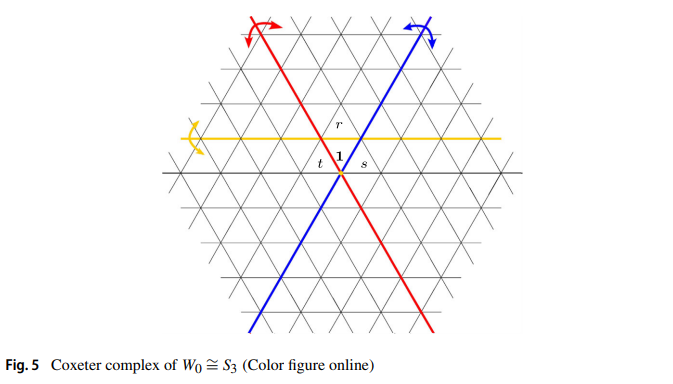
\includegraphics[scale=0.7]{Screenshot 2023-03-14 150033.png}\\
% \end{center}

% We call this finite Coxeter complex the boundary of the infinite Coxeter complex. We can represent the boundary as a tiling of an $(n-1)$-sphere, where $n$ is the dimension of the tiled space of the infinite Coxeter complex. So in this case, we can represent the boundary as a tiling of $S^1$.

Now we can make a very similar definition of a gallery for Coxeter complexes. We can view these as walks around the geometric realisation of the Coxeter complex, where we record the alcoves and panels we have crossed over. 

\begin{definition}\label{comb.gallery}
    Given a Coxeter complex \sg, a \ix{combinatorial gallery} is a sequence
    \[\gamma = (c_0,p_1,c_1,p_2,\hdots  ,p_n,c_n),\]
    where the $c_i$ are alcoves and the $p_i$ are panels of \sg, such that $p_i$ is contained in $c_{i-1}$ and $c_{i}$ for all $i-1,\hdots ,n$. The length of a combinatorial gallery $\gamma$ is $n+1$ - this counts how many alcoves there are in the sequence. Then $\gamma$ is \ix{minimal} if there does not exist a shorter gallery starting at $c_0$ and ending at $c_n$. 
\end{definition}

So a gallery is a path between $c_0$ and $c_n$ through alcoves, such that adjacent alcoves in the path share a commmon panel. This definition is the same as definition \ref{gallery}, but also encodes which panels we have crossed over in our walk. 

\begin{lemma}
    A Coxeter complex is connected.
\end{lemma}

\begin{proof}
    Given any two elements $x=s_{i_1}\hdots s_{i_n}$ and $y=s_{j_1}\hdots s_{j_m}$, we have a gallery
    \[s_{i_1}\hdots s_{i_n}\sim_{i_n}s_{i_1}\hdots s_{i_{n-1}}\sim_{i_{n-2}}\hdots \sim_{i_n} 1 \sim_{j_1}s_{j_1}\sim_{j_2}s_{j_1}s_{j_2}\sim_{j_3}\hdots\sim_{j_m}s_{j_1}\hdots s_{j_m}.\]
    So any two chambers are connected by a gallery.
\end{proof}


% \begin{lemma}
%     The automorphism group of the Coxeter complex is isomorphic to the Coxeter group, and this acts simple-transitively on the set of chambers.
% \end{lemma}

% \begin{proof}
%     $W$ acts on itself by left multiplication. This action clearly preserves the $i$-adjacency defined above. Now consider an automorphism which has a fixed chamber. Then all adjacent chambers must be fixed. This is because each rank 1 residue must have exactly two chambers, by definition. So, as Coxeter complexes are connected, we must fix the whole of the complex. So this action is simple-transitive. 
% \end{proof}

\subsection{Reflections and walls}
We next want to look at how the structure of the underlying Coxeter group appears in the Coxeter complex. We will see that the Coxeter group has a set of reflections which act exactly as reflections in the geometric realisation of the Coxeter complex, where these reflections are along the walls of the complex. 

\begin{definition}
    A \ix{reflection r} of $W$ is a conjugate of the generators of $W$. The wall $M_r$ of a reflection $r$ is the set of simplicies in the Coxeter complex which is fixed by $r$ when $r$ acts on the complex by left multiplication. Then $M_r$ is a subcomplex of codimension 1.
\end{definition}

By this definition, a panel lies in a wall $M_r$ if and only if it is fixed by the reflection $r$. 

\begin{example}
    In the case that the Coxeter complex is infinite and affine, the walls correspond to hyperplanes of the geometric realisation. 
\end{example}

\begin{theorem}
    There is a bijection between the set of reflections of a Coxeter group, and the set of walls in the corresponding Coxeter complex.
\end{theorem}

\begin{proof}
    Let $p$ be an $i$-panel of a chamber $x$. Then the unique reflection which fixes $p$ and interchanges $x$ and $xs_i$ is the map $r=xs_ix^{-1}$. So the map from reflections to walls is a bijection.
\end{proof}



%\subsection{Roots}

We now want to consider how the walls interact with our galleries, and the halfspaces defined by our walls.

\begin{definition}
    %A gallery $(c_0,\hdots ,c_k)$ \ix{crosses} $M_r$ if there is an $i$ such that $M_r$ interchanges $c_{i-1}$ and $c_i$. 
    A gallery $(c_0,p_1,\hdots ,p_k,c_k)$ \ix{crosses} a wall $M_r$ if there is a panel $p_i$ which lies in $M_r$, and $c_{i-1}\neq c_i$. 
\end{definition}

\begin{lemma}
    \begin{enumerate}
        \item Any minimal gallery does not cross a wall twice.
        \item Every gallery from two alcoves $x$ and $y$ have the same parity of crossings of any wall.
    \end{enumerate}
\end{lemma}


\begin{definition}
    Each hyperplane splits an apartment into two half-apartments called \ix{roots}. If $\alpha$ is one root, we denote the other corresponding root by $-\alpha$. 
\end{definition}


% \begin{definition}
%     A set of alcoves is called \ix{convex} if any minimal gallery between two alcoves of the set lies entirely within the set. 
% \end{definition}

% \begin{proposition}
%     \begin{enumerate}
%         \item Roots are convex.
%         \item Let $\alpha$ be a root, and let $x$ and $y$ be adjacent chambers with $x\in\alpha$ and $y\in -\alpha$. Then
%         \[\alpha =\{c\mid d(x,c)<d(y,c)\}.\]
%         \item There are bijections between the set of all reflections of a Coxeter group, the set of walls, and the set of pairs of opposite roots.
%     \end{enumerate}
% \end{proposition}

\begin{definition}\label{fold}
    A \ix{folding of W onto $\alpha$} is the map which fixes $\alpha$ and sends $-\alpha$ to $\alpha$ by relfecting across the defining wall of $\alpha$. 
\end{definition}

\begin{proposition}
    Consider any two chambers $x$ and $y$. Let $(x,p_1,x_1,\hdots ,x_{k-1,}p_k,y)$ be a minimal gallery from $x$ to $y$. Define $\beta_i$ to be the root which contains $x_{i-1}$ and which does not contain $x_i$. Then the $\beta_i$ are all distinct, and this set is all the roots which contain $x$ but do not contain $y$. So in particular, $d(x,y)=k$ is the size of the set of roots containing $x$ but not containing $y$. 
\end{proposition}

\begin{proposition}
    Given two chambers $x$ and $y$, a third chamber $z$ lies on a minimal gallery from $x$ to $y$ if and only if it is contained within every root which also contains $x$ and $y$. 
\end{proposition}


Let $R$ be a residue. Now we can define a map, called proj$_Rw$, which maps $w$ to the unique chamber of $R$ closest to $w$. 


\begin{proposition}
    Given a residue $R$ and a chamber $x\in R$, for any chamber $w$ there is a minimal gallery from $x$ to $w$ which passes through proj$_Rw$. 
\end{proposition}

% \begin{lemma}
%     Residues are convex.
% \end{lemma}

\begin{theorem}
    Given a gallery $\gamma$ of type $f$, $\gamma$ is minimal if and only if $f$ is reduced.
\end{theorem}


% \subsection{Finite Coxeter complexes}

% Now we assume that our group $W$ is finite, and so our Coxeter complex is also finite.

% \begin{definition}
%     The \ix{diameter}, diam$(W)$, of $W$ is the maximum distance between two chambers of the Coxeter complex. Two chambers are said to be \ix{opposite} if the distance between them is diam$(W)$.
% \end{definition}

% \begin{theorem}
%     \begin{enumerate}
%         \item diam$(W) = 1/2\ast \mid \{${roots of W}$\}\mid $. 
%         \item Two chambers are contained in no common root if and only if they are opposite.
%         \item For any given chamber, there is a unique opposite chamber.
%         \item Any chamber lies on a minimal gallery between two opposite chambers.
%     \end{enumerate}
% \end{theorem}


\section{Buildings}\label{4}

Now we are able to define buildings. These are just chamber systems with an added structure of a $W$-distance function, for some Coxeter group $W$. We will see that Coxeter complexes are buildings, but we can form more complicated buildings from our Coxeter complexes. In general, we will call each copy of a Coxeter complex in our building an \ix{apartment}. We will then look at some universal properties of buildings, and define two types of retractions of buildings onto an apartment. 

\begin{definition}
    Let $(W,S)$ be a Coxeter group with Coxeter matrix $M$, and let $I$ be an indexing set for the generators $S$ of $W$. A \ix{building of type M} is a chamber system $\Delta$ over $I$, such that each panel lies on at least two chambers, i.e.\ every $\{i\}$-residue contains at least two elements. We also require a $W$-distance function
    \[\delta:\Delta\times \Delta \to W,\]
    such that if $f$ is a reduced word in $S$, then we have that $\delta(x,y)=s_f$ if and only if there is a gallery of type $f$ between $x$ and $y$. We denote a building by $\Sigma=\Sigma(W,S)$. 
\end{definition}

\begin{lemma}\label{cox}
    Taking our $W$-distance function to be $\delta(x,y)=x^{-1}y$, Coxeter complexes are buildings.
\end{lemma}

\begin{proof}
    Consider a Coxeter group with presentation
    \[W=\langle s_i,i\in I\mid s_i^2=1,(s_is_j)^{m_{ij}}=1\rangle.\]
    Clearly, by definition, we have a chamber system over $I$. Now we need to show that each $\{i\}$-residue contains at least two elements. But that is trivial, as if $x$ is an element of an $\{i\}$-residue, then $x\cdot s_i$ is also an element of the same $\{i\}$-residue, and $x\neq x\cdot s_i$. 
    We also need to show that $\delta(x,y)=x^{-1}y$ is a valid $W$-distance function. But this comes from the observation that if $x=s_{i_1}\hdots  s_{i_k}$ and $y=s_{j_1}\hdots  s_{j_m}$, then there is a gallery of type $f=i_k\hdots  i_1j_1\hdots  j_k$. Then $s_f$ is exactly equal to $x^{-1}y$. 
\end{proof}

In fact, by the argument made in the proof of the above lemma, we conclude that each $\{i\}$-residue contains exactly two elements. We call this type of building a \ix{thin building}.


\subsection{Buildings and apartments}\label{apartments}
We can now form more complicated buildings by taking the union of Coxeter complexes. We can construct a chamber system $C$ which is the union of subsystems, all isomorphic to a given Coxeter complex formed from a Coxeter group $W$. We call each subsystem an \ix{apartment}. We require that every pair of chambers lie in a common apartment. We assume that, for any two apartments $A$ and $A'$ which contain a common chamber $x$ and a common chamber or panel $y$, there is an isomorphism $A\to A'$ which fixes $x$ and $y$.  

\begin{theorem}
    The above construction gives a building, with $W$-distance function $\delta(x,y)$ defined by the $W$-distance function on any apartment containing $x$ and $y$. 
\end{theorem}

\begin{proof}
    This is clearly a chamber system over the set $I$, where $I$ is the indexing set of the Coxeter group generators. We first need to prove that each $\{i\}$-residue contains at least two chambers. But this follows from the fact that we are taking the union of Coxeter complexes, and this statement holds on each apartment by lemma \ref{cox}. 

    We now note that we are assuming that any two apartments are isomorphic, so the $W$-distance function is well-defined. So let us assume, for two chambers $x$ and $y$, that $f$ is a reduced word and $\delta(x,y)=s_f$. Now this means that, given any apartment containg both $x$ and $y$, there is a gallery of type $f$ from $x$ to $y$. 

    Now we need to show the converse. We need to show that if there is a gallery of type $f$ from $x$ to $y$ which is reduced, then $\delta(x,y)=s_f$. We prove this by induction on the length of $f$. 

    For the base case, if $f=i$ then $x$ and $y$ are $i$-adjacent, and so they are $i$-adjacent in any apartment containing them both. So then $\delta(x,y)=s_i$.

    Now assume that there is a reduced gallery of type $f=gi$ from $x$ to $y$. Let $A$ be an apartment containing both $x$ and $y$. Let $p$ be the last panel in our gallery, and $y'$ the second to last alcove in the gallery. So $p$ will have type $i$. Now, by induction, $\delta(x,y')=s_g$. This implies that there is a gallery $\gamma$ of type $g$ from $x$ to $y'$ in some apartment, say $A'$.
    
    Now we know, by the definition in section \ref{apartments}, that there is an isomorphism $\phi : A\to A'$ which fixes $x$ and $p$. So now consider the gallery $\gamma$ under the map $\phi$. This gives us a gallery which starts at $\phi(x)=x$ and ends at a gallery which has $p$ as one of its panels. Also, this gallery has type $g$. Hence, we can create a new gallery $(\phi(\gamma),y)$ of type $f=gi$ from $x$ to $y$. This finishes our proof.
\end{proof}


\begin{example}
    Example \ref{AnK} is an example of a building constructed this way. Here, our apartments are copies of 6-cycles, which are copies of the Coxeter complex for $A_2$. This is why this building is called the $A_2(\mathbb{F}_2)$ building. Clearly any two chambers are contained in a common apartment. 
    \begin{center}
        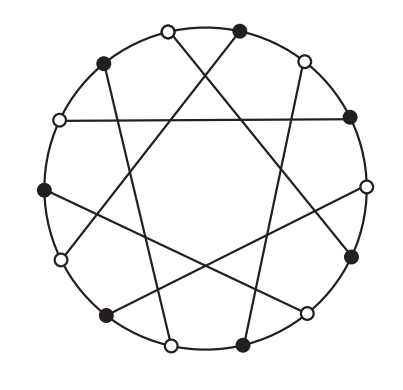
\includegraphics[scale=0.5]{Screenshot 2023-03-16 131651.png}\\
    \end{center}
\end{example}


\subsection{Properties of buildings}
Some key properties of buildings are as follows:
\begin{enumerate}
    \item $\Delta$ is connected.
    \item $\delta$ is surjective.
    \item $\delta(x,y)=\delta(y,x)^{-1}$.
    \item $\delta(x,y)=s_i$ if and only if $x\neq y$ and $x\sim_i y$.
    \item For $i\neq j$, $i$- and $j$-adjacency are mutually exclusive.
    \item For chambers $x$ and $y$, if there is a gallery from $x$ to $y$ of type $f$, and $f$ is homotopic to $g$, then there is a gallery from $x$ to $y$ of type $g$. 
    \item A gallery if minimal if and only if its type is reduced.
    \item If there is a gallery of type $f$ from $x$ to $y$, and $f$ is reduced, then this gallery is unique.
\end{enumerate}



\begin{theorem}
    Any $J$-residue is a building of type $M_J$. 
\end{theorem}

\begin{proof}
    We note that we only need to show that the $W_J$-distance function is well-defined, as the other properties of a building are obvious. So in particular, we need to show that $\delta(x,y)\in W_J$ for all $x,y$ in the same $J$-residue. Consider a shortest $J$-gallery $\gamma$ between $x$ and $y$, and let $f$ be its type. Then $f$ is a word in $\{s_i\mid i\in J\}$. Assume that $f$ is not reduced. Then $f$ must be homotopic to some shorter word $g$ in $\{s_i\mid i\in J\}$. So by our sixth observation above, there must be a gallery from $x$ to $y$ with type $g$. This contradicts $\gamma$ being a shortest $J$-gallery between $x$ and $y$. So $F$ is reduced, and hence $\delta(x,y)\in W_J$. 
\end{proof}


% The next theorem allows us to conclude that any two chambers have a common apartment. The proof of this theorem can be found in \cite[p.31]{RON}.

% \begin{theorem}\label{isometry}
%    Any isometry from a subset of $W$ into $\Delta$ can be extended to an isometry of $W$ into $\Delta$.
% \end{theorem}


% \begin{corollary}
%     Any two chambers lie in a common apartment.
% \end{corollary}

%\begin{theorem}
  %  Apartments are convex.
%\end{theorem}

\section{Retractions of buildings}\label{5}

%Now we can use our definition in section \ref{apartments} to define retractions of a building. These are maps from a building made of many apartments, onto one of its apartments. By our definition of buildings constructed from Coxeter complexes, we can see that an isometry from $W$ to a building $\Delta$ is uniquely determined its image and where the identity element $1\in W$ is sent. 

We can now define retractions of buldings. This is a map from the building, onto one of its apartments. As we will see in section \ref{retract}, there is a natural connection between retractions and the shadows of galleries. This gives us a motivation for studying the shadows of galleries. 

\begin{definition}
    Let $A$ be a chosen apartment in a building $X$, and let $c\in A$ be an alcove. We define the \ix{retraction from X to A based at c} as the map $r_{A,c}:X\longrightarrow A$ where we send any alcove $d$ to the unique alcove $e$ in $A$ such that $\delta(c,d)=\delta_A(c,e)$. 
\end{definition}

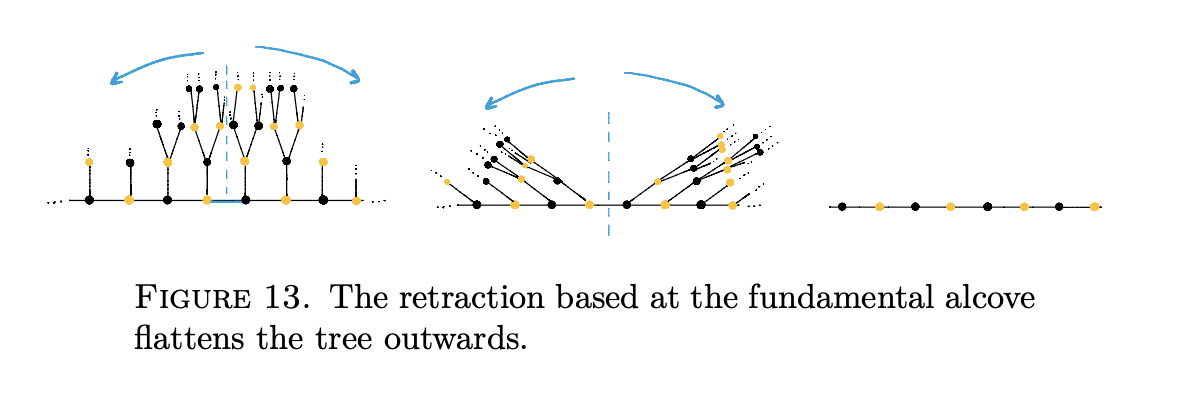
\includegraphics[scale=0.7]{Screenshot 2023-02-15 at 13.32.45.png}\\


We now want to define the concept of a retraction from infinity. The idea here is you pick a Weyl chamber, and so a chamber in the boundary, and effectively fold away from this direction. We do this by employing the retraction from an alcove, but this alcove must change depending on the alcove we are trying to retract. This alcove must be far enough away, and in the direction of the chamber at infinity. Take $w_0$ as the alcove at the tip of the Weyl chamber $C$, where we are considering the finite Coxeter complex within the affine complex which contains the fixed alcove 1. We also take as $t$ the element which maps the finite complex onto its next copy in the direction of the Weyl chamber containing 1. 

\begin{centering}
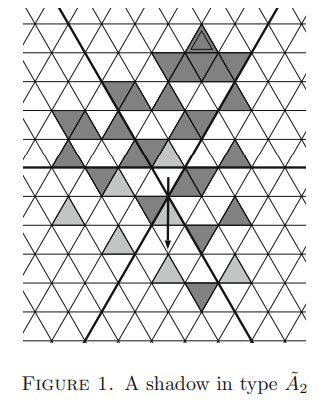
\includegraphics[scale=0.5]{Screenshot 2023-03-28 114049.png}\\
\end{centering}
\tr{I need to create this picture to show what $w_0$ we are picking.}

In the example of $\tilde{A}_2$, we take as $t$ the element $s_0s_1s_2s_1$. This translates the hexagon onto the next hexagon in the direction of the Weyl chamber containing 1. 

\begin{definition}
    Let $A$ be a chosen apartment in an affine building $X$, and let $C\in \partial A$ be a chamber at infinity of the apartment. We define the \ix{retraction from X to A based at C} as the map $\rho_{A,C}:X\longrightarrow A$ which, for any alcove $d$, of length $l(d)$, we take the alcove $c=w_0t^{l(d)}$, as defined above. Then $\rho_{A,C}(d)=r_{A,c}(d)$.
     %which sends an alcove $d$ to its image under the isomorphism from the apartment containing both $d$ and a Weyl chamber representing $C$ to $A$. 
    
\end{definition}
The idea here is that for any alcove we are wanting to retract, we are wanting to take an alcove which is 'far enough away' in the direction of the chosen Weyl chamber. 

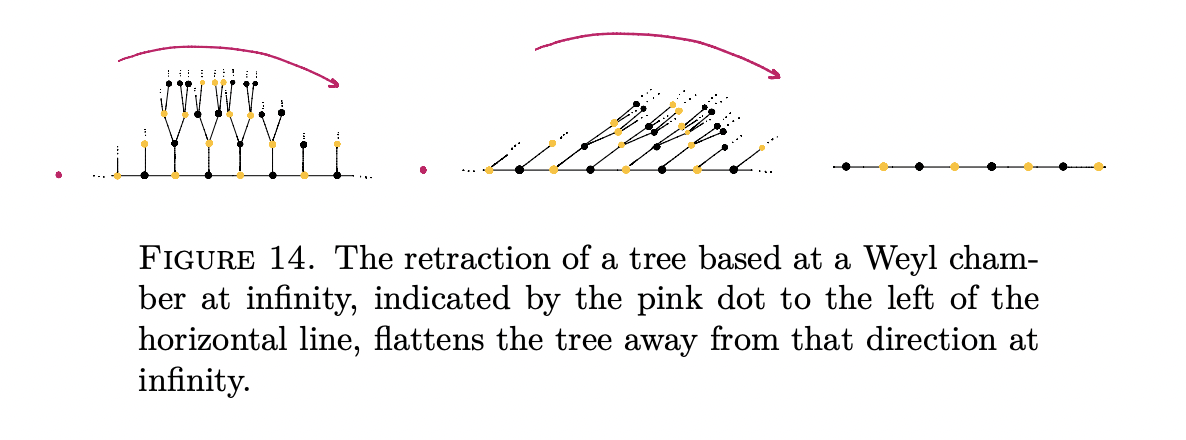
\includegraphics[scale=0.7]{Screenshot 2023-02-15 at 13.31.58.png}


\section{Orientations of buildings}\label{6}

We want to consider an orientation on the panels of our buildings. Ultimately, we want to define foldings of galleries, and we only want to consider postive foldings with respect to some orientation.


\begin{definition}
    An \ix{orientation} $\phi$ of a building $\Sigma$ is a map from the set of pairs $(p,c)$, where $p$ is a panel and $c$ is an alcove containing $p$, to the set $\{+1,-1\}$. If $\phi (p,c)=+1$, then we say that $c$ is on a $\phi$-\ix{positive side} of $p$, otherwise we say that $c$ is on a $\phi$-\ix{negative side}. 
\end{definition}


\begin{example}
    The trivial positive orientation is the map which sends all pairs to $+1$. Similarly, the trivial negative orientation is the map which sends all pairs to $-1$. 
\end{example}

Often, we do not want to have orientations which locally behave like trivial orientations. Hence, we define the following concepts:

\begin{definition}
    Given an orientation $\phi$ of \sg, we have
    \begin{enumerate}
        \item $\phi$ is \ix{locally non-negative} if, for each panel, there is at least one alcove which is on the $\phi$-positive side.
        \item $\phi$ is \ix{locally non-trivial} if, for each panel, there is exactly one alcove which is on the $\phi$-positive side.
    \end{enumerate}
\end{definition}


There is a natural action of $W$ on the set of all possible orientations of \sg, induced by the action of $W$ on on the alcoves and panels. It is defined as 
\[(x\cdot\phi)(p,c):=\phi(x^{-1}p,x^{-1}c).\]

\begin{definition}
    Given an orientation $\phi$ of \sg, we say that $\phi$ is \ix{wall consistent} if, given any wall $H$, for all pairs $c,d$ of alcoves which lie in the same halfspace of $H$, with panels $p$ and $q$ lying in $H$, we have that $\phi(p,c)=\phi(q,d)$. If our orientation is wall consistent, we can then define the \ix{positive side} $H^{\epsilon}$ of $H$ as the half-space such that all alcoves $c$ in $H^{\epsilon}$ have $\phi(p,c)=+1$ for all panels of $c$. Then the \ix{negative side} is defined similarly.
\end{definition}

We want to look at several natural ways to orient a Coxeter complex. First, we will look at an orientation which is derived from either a choice of alcove, or a choice of panel. This orientation works for any Coxeter group.

\begin{definition}
    Choose a fixed alcove $c$ in \sg. Now given any alcove $d$, and panel $p$, we define their orientation as $\phi(p,d)=+1$ if and only if $c$ and $d$ lie in the same side of the wall which is spanned by $p$. We call this orientation the \ix{alcove orientation towards c}.
\end{definition}


\begin{definition}
    Choose a fixed simplex $b$ in \sg. Now given any alcove $c$, and panel $p$ in $c$, we define their orientation as $\phi(q,c)=+1$ if and only if either $c$ and $b$ lie in the same side of the wall $H$ containing $p$, or if $b$ lies inside $H$. We call this orientation the \ix{simplex orientation towards b}.
\end{definition}
\begin{example}
    Here we see two simplex orientations of an $A_2$ Coxeter complex. In this complex, the alcoves are edges, and the panels are vertices. The walls in this picture are the sets of pairs of points which are diagonal each other. This is because the map which switches the neighbouring panels fixes the point in between and the opposite point. 
\end{example}
\begin{center}
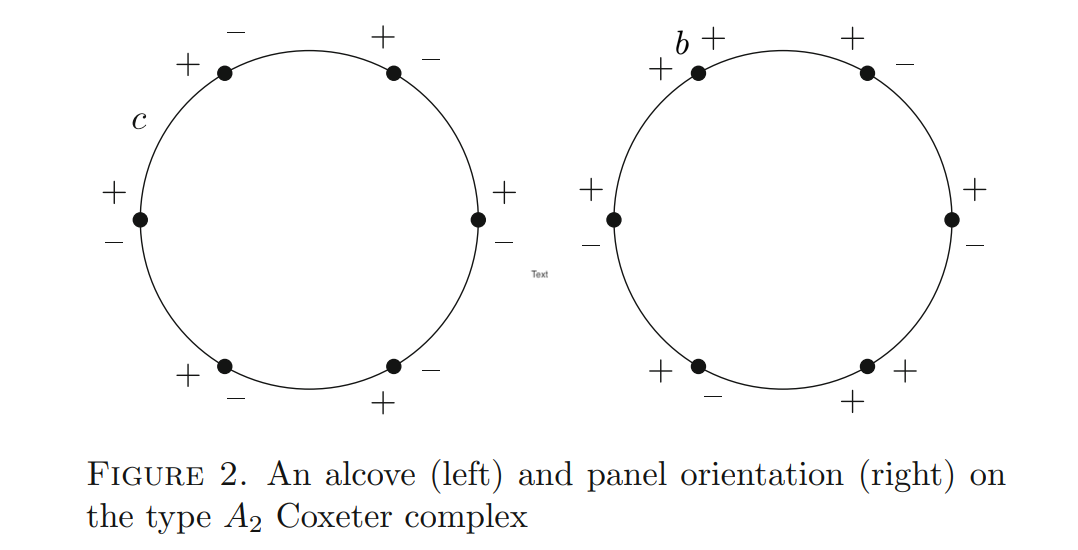
\includegraphics[scale=0.5]{Screenshot 2023-02-03 102201.png}\\
\end{center}
\begin{lemma}
    Consider a Coxeter group $(W,S)$ with Coxeter complex \sg. We have the following:
    \begin{enumerate}[(i)]
        \item If $\phi$ is a simplex orientation of \sg, then $\phi$ is wall consistent and locally non-negative.
        \item If $\phi$ is an alcove orientation of \sg, then $\phi$ is wall consistent and locally non-trivial.
    \end{enumerate}
\end{lemma}

\begin{proof}
    (i) Let $b$ be the simplex defining the orientation, and consider a wall $H$ in our Coxeter complex. First let us consider the case in which $b$ lies inside $H$. Then, by definition of the simplex orientation, both sides of the wall are defined to be positive. So any two alcoves, and any respective panels, lying in the same root of $H$ will have the same orientation. So this root satisfies the conditions of wall consistency, and both sides are defined as positive so it is locally non-negative. 
    
    Now assume that $b$ does not lie in $H$, so $b$ lies in exactly one root of $H$. Then this side of the wall is the positive side, and any two alcoves, and any respective panels, in this root are given a positive orientation. Similarly, any two alcoves, and any respective panels, in the other root are given a negative orientation. So again, this wall satisfies the conditions of wall-consistency, and both sides are defined as positive so it is locally non-negative. 

    (ii) An alcove orientation is a type of simplex orientation, so part (i) implies that $\phi$ is wall consistent. Now considering the cases from part (i), we can never be in the first case. This is because an alcove has one higher dimension whan a wall, and so an alcove can never fully lie within a wall. So therefore we are always in case two, and so by the same argument as part (i), we conclude that $\phi$ is locally non-trivial. 
\end{proof}

\subsection{The affine case}

Now we restrict to the case that our Coxeter complex $\Sigma$ is affine. To define an orientation on \sg, we choose a chamber at infinity.

If $\phi$ is a wall consistent orientation, then, given two chambers $c,d$ which share a common panel $p$, $c$ and $d$ are given the same orientation if they lie in the same half-space of the hyperplane spanned by $p$. This amounts to picking a positive side of the hyperplane.

However, we did not have to pick these positive sides in any consistent way. 

\begin{definition}
    Let $\phi$ be a wall consistent orientation of an affine Coxeter complex. We say that $\phi$ is \ix{periodic} if, given two parallel hyperplanes $H_1,H_2$ and corresponding half-spaces $H_1^{\epsilon},H_2^{\epsilon}$, if $H_1^{\epsilon}\subset H_2^{\epsilon}$, then $H_1^{\epsilon}$ is positive if and only if $H_2^{\epsilon}$ is positive. 
\end{definition}

\begin{example}
    If $\phi$ is a trivial orientation on an affine Coxeter complex, then $\phi$ is periodic. 
\end{example}

\begin{example}
    Simplex orientations are not periodic, as, for every set of parallel hyperplanes, we can find pairs of representatives which have the simplex on different sides.
\end{example}

If $\phi$ is a periodic orientation, then we have a natural orientation induced on the boundary. Similarly, if we have an orinetation defined on the boundary of a Coxeter complex, then we have a periodic orientation on the Coxeter complex which induces this orientation. 

\begin{lemma}\cite[p.125]{SHA}
    Given a periodic orientation $\phi$ on an affine Coxeter complex \sg, there is an induced wall-consistent orientation $\partial\phi$ on the boundary complex $\partial\Sigma$. Now if $\phi$ is locally non-negative or non-trivial, so is $\partial\phi$. 
\end{lemma}

\begin{proof}
    Consider a wall $M$ in the boundary $\partial\Sigma$. This corresponds to a set of parallel walls in $\Sigma$. Consider a chamber $a\in \partial\Sigma$, which has a panel $p$ lying in $M$. Now we can find a Weyl chamber $C_a$ of $\Sigma$ which represents $a$. This has a bounding wall $H_M$ in the set of parallel walls corresponding to $M$. Let $c$ be the alcove at the tip of $C_a$. So $c$ has a panel $q$ which lies in $H_M$. We now define the orientation of the boundary by 
    \[\partial \phi (a,p)= \phi (c,q).\]
    This is well-defined as $\phi$ is periodic, so the choice of $C_a$ does not affect the orientation. Also, as $\phi$ is periodic, this orientation is wall-consistent. 
    If $\phi$ is locally non-negative, then given a panel $q$ of $\Sigma$, we can find an alcove $d$ such that $\phi(d,q)=+1$. Then under the projection map from $\Sigma$ to the boundary $\partial\Sigma$, we get a chamber $a$ and panel $p$ such that $\partial\Sigma(a,p)=+1$. So $\partial\phi$ is locally non-negative. The same argument can be made to show that if $\phi$ is locally non-trivial, then $\partial\phi$ is also locally non-trivial. 
\end{proof}


\begin{lemma}
    Given a wall-consistent orientation $\phi$ of the boundary complex $\partial\Sigma$, there exists a unique periodic orientation $\tilde{\phi}$ of \sg which induces the orientation $\phi$. 
\end{lemma}

\begin{proof}
    Let $H$ be a wall in $\Sigma$. Given a wall $H^\epsilon$ of $H$, we define $H^\epsilon$ to be the positive side of $H$ if the corresponding root $\partial H^\epsilon$ is the positive side of the wall $\partial H$ with respect to the orientation $\phi$. Otherwise we define $H^\epsilon$ to be the negative side of $H$. This is well-defined as $\phi$ is wall-consistent. This definition also uniquely defines the orientation $\tilde{\phi}$. 
\end{proof}

\begin{definition}
    Let $\sigma$ be a chamber of the boundary $\Delta$ of a Coxeter complex \sg. Then we form an orientation $\phi_{\sigma}$ on the boundary $\Delta$. The \ix{Weyl chamber orientation} on $\Sigma$ is the oritentation on $\Sigma$ which induces $\phi_{\sigma}$. 
\end{definition}


\section{Folded galleries}\label{7}

Next, we will consider folded galleries in a Coxeter complex. These are galleries which have a repeated chamber. We will see how we can define a type of a gallery. This encodes the types of all the panels we crossed over or touched in our gallery. We will also define the decorated type. This also encodes the location of folds in our gallery. The decorated type, along with the footprint function and starting alcove, can be used to calculate the end alcove of our gallery. 

\subsection{Definitions}


\begin{definition}
    Given a gallery $\gamma$ of \sg, we say that $\gamma$ is \ix{folded} (or \ix{stammering}) if, within $\gamma$, we can find an index $i$ such that $c_i=c_{i-1}$. Then we say that $\gamma$ has a \ix{fold} at panel $p_i$. Otherwise, we say that $\gamma$ is \ix{unfolded} (or \ix{non-stammering}).  
\end{definition}

\begin{definition}
    Given a gallery $\gamma$, define the set F$(\gamma)$ to be the subset of $\{1,\hdots ,n\}$ such that $i\in$ F$(\gamma)$ if and only if $\gamma$ has a fold at panel $p_i$. 
\end{definition}

To represent a gallery, we draw a path which passes through every chamber and panel in the gallery of the geometric representation of our Coxeter complex. We draw an arrow towards the end alcove of our gallery. 

\begin{center}
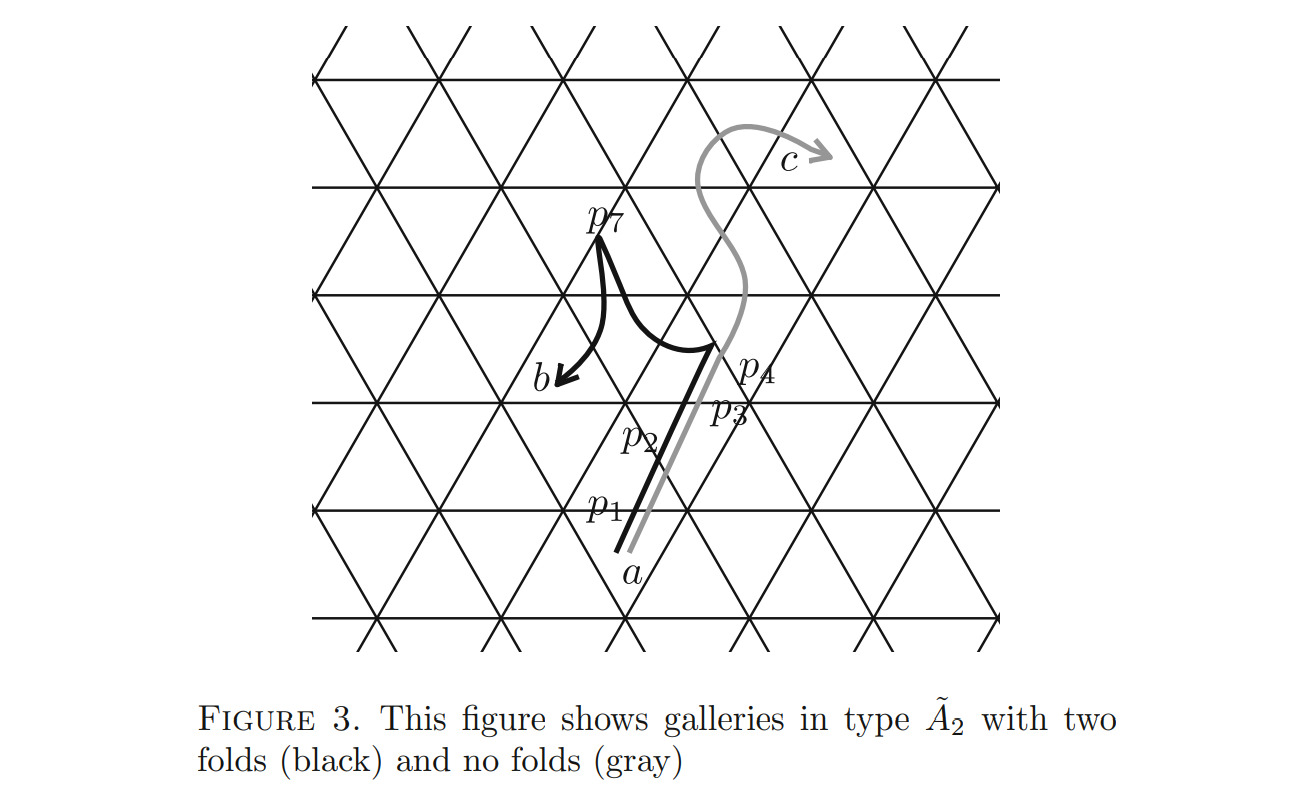
\includegraphics[scale=0.4]{Screenshot 2023-02-03 111653.png}\\
\end{center}

\begin{definition}
    Given a gallery $\gamma$ in \sg, and an orientation $\phi$, we say that $\gamma$ is \ix{positively folded} with respect to $\phi$ if, whenever $\gamma$ is folded at position $i$, $\phi(p_i,c_i)=+1$.  We can similarly define \ix{negatively folded}.
\end{definition}

We note that, as $W$ has a natural left action on \sg, $W$ also acts on the set of galleries in \sg. For instance, $x\in W$ sends $\gamma = (c_0,p_1,c_1,\hdots ,p_n,c_n)$ to the gallery $\gamma = (xc_0,xp_1,xc_1,\hdots ,xp_n,xc_n)$. 

\begin{lemma} 
    Consider an affine Coxeter system $(W,S)$ with a Coxeter complex \sg. Let $a$ be a chamber in the boundary complex $\partial\Sigma$. Now a gallery $\gamma$ is $\phi_a$-positively folded if and only if $x\cdot \gamma$ is $\phi_a$-positively folded. So the action of $W$ on $\partial\Sigma$ preserves the condition of being '$\phi_a$-positively folded'.
\end{lemma}

\subsection{Galleries and words}

We can now define the type and decorated type of a gallery. Note that here we use tilde notation to denote a decorated word, but in other texts, such as \cite{SHA}, they use hat notation to denote the decorated word.

\begin{definition}
    Consider a gallery $\gamma = (c_0,p_1,c_1,\hdots ,p_n,c_n)$. Let panel $p_i$ of $\gamma$ have type $s_{j_i}\in S$. We define its \ix{type} $\tau(\gamma)$ as the word 
    \[\tau(\gamma):=s_{j_1}\hdots s_{j_n}.\]
    We denote by $\Gamma_{\phi}^+(w)$ the set of all $\phi$-positively folded galleries which have type $w$. 
\end{definition}

\begin{definition}
    The \ix{decorated type} $\tilde\tau(\gamma)$ of a gallery $\gamma = (c_0,p_1,c_1,\hdots ,p_n,c_n)$ is the decorated word
    \[\tilde\tau(\gamma):= s_{j_1}\hdots \tilde{s_{j_i}}\hdots s_{j_n},\]
    where we place a tilde on the elements $s_{j_i}$ of the word which correspond to a fold $c_{i-1}=c_i$ of the gallery. We denote by $\Gamma_{\phi}^+(\tilde{w})$ the set of all $\phi$-positively folded galleries which have decorated type $\tilde{w}$.
\end{definition}


\begin{lemma}\cite[p.128]{SHA}
    Let $c_0$ be a fixed alcove in our Coxeter complex \sg. 
    \begin{enumerate}[(i)]
        \item There is a bijection between words in $S$ and unfolded galleries starting at $c_0$.
        \item There is a bijection between decorated words in $S$ and gallleries starting at $c_0$. 
    \end{enumerate}
\end{lemma}

\begin{proof}
    Given a word $s_1\hdots s_n$ in $S$, we can define an unfolded gallery starting at $c_0$ by multiplying $c_0$ by $s_1$, and in general define $c_i$ by multiplying $c_{i-1}$ by $s_{i}$, and set $p_i$ to be the unique panel contained in both $c_{i-1}$ and $c_i$. This gives our bijection for part (i). 
    Now given a decorated word in $S$, we can define a general gallery by multiplying $c_{i-1}$ by $s_{i}$, as above, if $s_{i}$ is not decorated. If $s_{i}$ is decorated, then let $c_i=c_{i-1}$, and let the panel $p_i$ be the unique panel of $c_i$ which has type $s_i$. This gives the bijection for part (ii). 
\end{proof}

The next lemma gives some easy results from the definitions of type and decorated type. 

\begin{lemma}\cite[p.128]{SHA}
    Let $\gamma$ be a gallery. Then
    \begin{enumerate}
        \item $F(\gamma)=\emptyset$ if and only if $\tau(\gamma)=\tilde{\tau}(\gamma).$
        \item $\gamma$ is minimal if and only if $F(\gamma)=\emptyset$ and $\tau(\gamma)$ is reduced.
    \end{enumerate}
\end{lemma}

We want to be able to characterise the last alcove in a gallery. We do this by constructing another gallary which removes any folds from our original gallery. This leads to an unfolded gallery which has shorter length than the original gallery.

\begin{definition}
    Consider a gallery $\gamma = (c_0,p_1,c_1,\hdots ,p_n,c_n)$ in \sg. We create a new gallery, called the \ix{footprint} ft$(\gamma)$ \ix{of} $\gamma$, by deleting all pairs $p_i,c_i$ such that the letter $s_i$ has a hat in $\hat{\tau}(\gamma)$. 

\end{definition}

\begin{center}
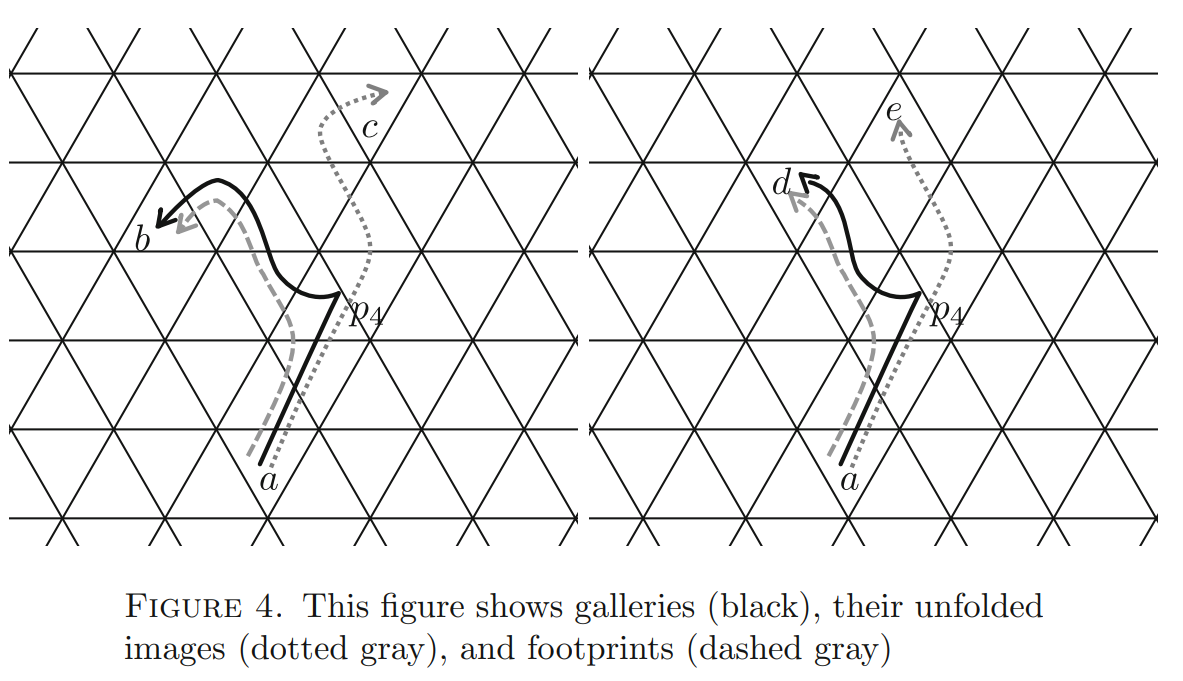
\includegraphics[scale=0.4]{Screenshot 2023-02-03 133522.png}\\
\end{center}

\begin{lemma}
    We can calculate the final alcove of a gallery as the element $c_n=c_0\cdot w$, where $w=\tau(\text{ft}(\gamma))$.
\end{lemma}

\begin{proof}
    The footprint of a gallery is exactly the gallery achieved by deleting repeated alcoves and the corresponding panels. So we are left with a gallery ft$(\gamma)=(c_o=d_0,q_1,d_1,\hdots ,q_m,d_m=c_n)$. Now $d_i$ is exactly defined as the alcove obtained by multiplying $d_{i-1}$ by $s_i$, where $s_i$ is the type of the panel $q_i$. So, by induction, $d_m$, which equals $c_n$, can be calculated by multiplying $d_0=c_0$ by the type of ft$(\gamma)$. 
\end{proof}

\subsection{Folding and unfolding galleries}

Now we have defined galleries, and in particular folded galleries, we want to be able to create folded galleries ourselves from unfolded galleries. We do this in a natural way, where folding along a panel leads to a reflection of the rest of the gallery with respect to that panel. For instance, this figure shows foldings in the 4th and 7th panel of the given gallery, and also illustrates that foldings are commutative - a fact that we will formally prove.
\begin{center}
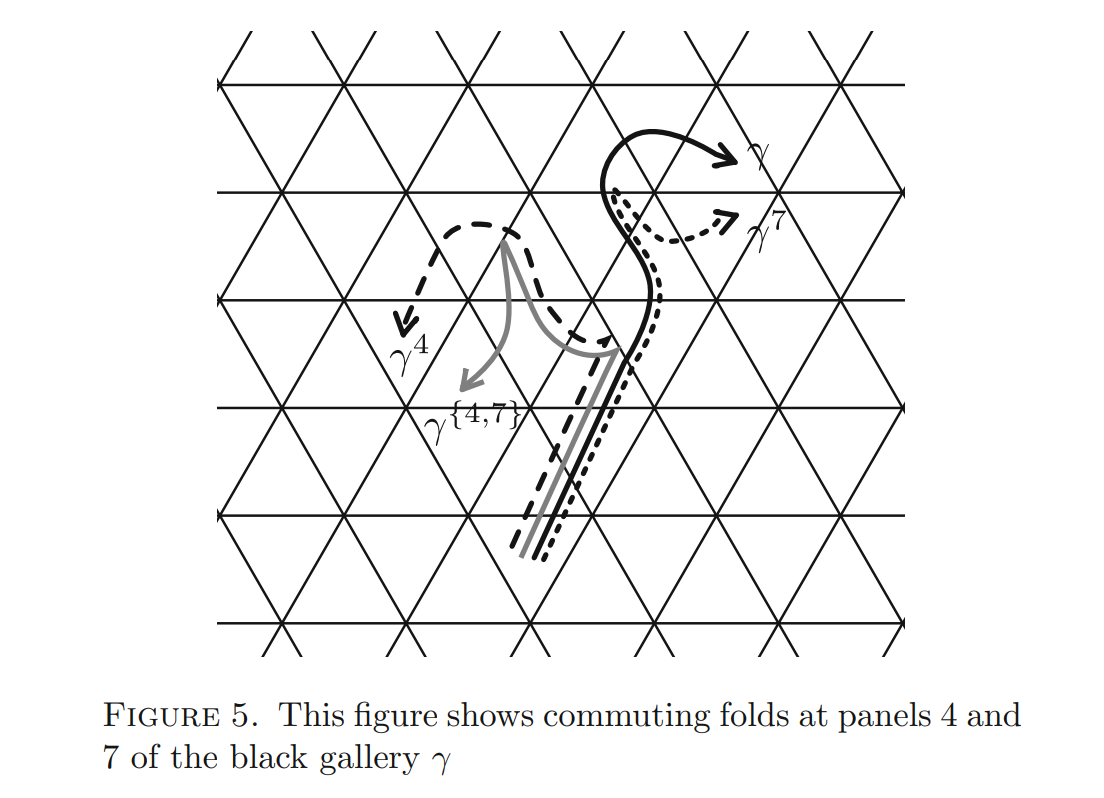
\includegraphics[scale=0.4]{Screenshot 2023-02-03 153412.png}\\
\end{center}

\begin{definition}
    Consider a gallery $\gamma = (c_0,p_1,c_1,\hdots ,p_n,c_n)$. Let $H_i$ be the wall containing the panel $p_i$, and let $r_i$ be the reflection across $H_i$. For $i=1,\hdots ,n$, let
    \[\gamma^i:=(c_o,p_1,\hdots ,p_i,r_ic_i,r_ip_{i+1},r_ic_{i+1},\hdots ,r_ip_n,r_ic_n).\]
    If $\gamma$ was folded at panel $p_i$, we call $\gamma^i$ a \ix{unfolding of }$\gamma$ at $p_i$. Otherwise, we call it a \ix{folding}.
\end{definition}

Compare this definition of folding to definition \ref{fold}. We see that this definition is a restriction of the map defined in definition \ref{fold} to the gallery we are folding. 
\begin{lemma}
    For all $i=1,\hdots ,n$, $\tau(\gamma)=\tau(\gamma^i)$. So folding and unfolding does not change the gallery type. Also, $(\gamma^i)^i=\gamma$.
\end{lemma}

\begin{proof}
    This is just a result of the definition of the type of a panel, which is invariant under reflections along walls. Also, we note that $r_ir_i=1$, as reflections are self-inverse, so applying a fold twice at panel $p_i$ will first achieve $(c_o,p_1,\hdots,p_i,r_ic_i,r_ip_{i+1},r_ic_{i+1},\hdots ,r_ip_n,r_ic_n)$, and will then achieve $(c_o,p_1,\hdots ,p_i,r_ir_ic_i,r_ir_ip_{i+1},r_ir_ic_{i+1},\hdots ,r_ir_ip_n,r_ir_ic_n)=(c_0,p_1,\hdots ,p_n,c_n)$. Hence, $(\gamma^i)^i=\gamma$.
\end{proof}

\begin{lemma}
    For all $i,j=1,\hdots,n$, $(\gamma^i)^j=(\gamma^j)^i$, i.e.\ foldings are commutative.
\end{lemma}

\begin{proof}
    As we have already dealt with the case that $i=j$, we can assume that $i<j$. Let $r$ be the reflection along the wall containing $p_i$, and let $t$ be the reflection along the wall containing $p_j$. Then we have, by the definition of (un)-folding,
    \[(\gamma^j)^i=(c_0,p_1,c_1,\hdots,c_{i-1},p_i,rc_i,\hdots ,rp_j,rtc_j,\hdots ,rtc_n).\]
    Also, if we let $u$ be the reflection along the wall containing $rp_j$, we have
    \[(\gamma^i)^j=(c_0,p_1,c_1,\hdots ,c_{i-1},p_i,rc_i,\hdots ,rp_j,urc_j,\hdots ,urc_n).\]
    Let us calculate the maps $r$, $t$ and $u$. Given a panel $p$ of an alcove $c$, the reflection along the wall containing $p$ is given by the multiplication map $c\tau(p)c^{-1}$. Hence,
    \[r=c_{i-1}\tau(p_i)c_{i-1}^{-1}, t=c_{j-1}\tau(p_j)c_{j-1}^{-1}, \textnormal{ and } u=(rc_{j-1})\tau(rp_j)(rc_{j-1})^{-1}.\]
    Now by a previous lemma, reflections preserve type, so we have that $\tau(rp_j)=\tau(p_j)$. Then
    \[\begin{aligned}
        ur & =(rc_{j-1})\tau(rp_j)(rc_{j-1})^{-1}c_{i-1}\tau(p_i)c_{i-1}^{-1}\\
           & =r(c_{j-1}\tau(p_j)c_{j-1}^{-1})(c_{i-1}\tau(p_i)c_{i-1}^{-1})(c_{i-1}\tau(p_i)c_{i-1}^{-1})\\
           & = r(c_{j-1}\tau(p_j)c_{j-1}^{-1})\\
           & =rt.
    \end{aligned}\]
    Therefore $ur=rt$, and hence $(\gamma^j)^i=(\gamma^i)^j$.
\end{proof}

Because of this property, we are able to define a \ix{multifolding} with respect to a subset $I$ of $\{1,\hdots ,n\}$ as the (un-)foldings $\gamma^I$. Now multifoldng does not affect the type. Then the set of folds of $\gamma^I$ will be the symmetric difference of the folds of $\gamma$ and $I$. In particular, if $I$ and $J$ are subsets of $\{1,\hdots ,n\}$, $(\gamma^I)^J=\gamma^{I\Delta J}$. The following corollary now follows.

\begin{corollary}
    Given any gallery $\gamma$, there is a subset $I\subset \{1,\hdots ,n\}$ such that $\gamma^I$ is unfolded, and $\gamma$ and $\gamma^I$ have the same type.
\end{corollary}


Now we fix an alcove of our Coxeter complex, and call this 1. Then, for any word $w$ with elements in $S$, we let $\gamma_w$ be the unique unfolded gallery which has type $w$ and starts at 1. Now we write
\begin{enumerate}
    \item $\gamma \rightharpoonup \eta$ if $\gamma$ and $\eta$ are galleries such that $\eta = \gamma^I$ for some index set $I$, i.e.\ there is a folding of $\gamma$ which gives $\eta$.
    \item $w\rightharpoonup u$ if $w$ and $u$ are words in $S$ such that there is a folding of $\gamma_w$ which has footprint $u$.
    \item $w\rightharpoonup x$ if $x$ is an element of $W$ such that there is a folding of $\gamma_w$ which has end alcove $c_x$. 
\end{enumerate}
We denote by $A\stackrel{\phi}{\rightharpoonup} B$ if the respective gallery is $\phi$-positively folded.


\subsection{Braid invariant orientations}

Two reduced words in $S$ represent the same element in the Coxeter group if and only if they differ by a squence of braid moves. A braid move replaces a subword $s_is_j\hdots $ of length $m_{ij}$ with the string $s_js_i\hdots $, again of length $m_{ij}$. We want to define the concept of braid invariant orientations, so we can later conclude that, if we have a braid invariant orientation, our shadows of a gallery do not depend on the chosen word of $S$ representing the end alcove. 

\begin{definition}
    Consider a Coxeter system $(W,S)$ and a corresponding Coxeter complex \sg. Let $\phi$ be an orientation on \sg. Then we say that $\phi$ is \ix{braid invariant} if, given any two braid equivalent words $w,w'$ in $S$ and any $x\in W$, $w\stackrel{\phi}{\rightharpoonup} x$ if and only if $w'\stackrel{\phi}{\rightharpoonup} x$. Then if $y\phi$ is braid invariant for all $y\in W$, $\phi$ is called \ix{strongly braid invariant}. 
\end{definition}

For instance, trivial orientations are strongly braid invariant, but these orientations are not very interesting. The following proposition gives us a large family of orientations which are braid invariant. A proof of this proposition can be found in \cite[pp.135-138]{SHA}.

\begin{proposition}
    Weyl chamber orientations are braid invariant.
\end{proposition}


\section{Shadows}\label{8}
Now we have defined orientations on a Coxeter complex, and looked at folding and unfolding galleries, we can define the shadow of a given gallery. This is exactly the set of end alcoves which can be reached by positively folding the gallery. 


\begin{definition}
    Consider a Coxeter system $W$ and an orientation $\phi$ on the Coxeter complex \sg\W. Let $w$ be a word is $S$. The \ix{shadow} of $w$ with respect to $\phi$ is the set 
    \[\textnormal{Sh}_\phi(w):=\{u\in W\mid w\stackrel{\phi}{\rightharpoonup} u\}.\]
    If $\phi$ is braid invariant, we can define Sh$_\phi(x)=$Sh$_\phi(w)$, where $w$ is any reduced expression of $x\in W$. If we have the Weyl chamber orientation $\phi_a$ with $a\in W_0$, the \ix{regular shadow} of $x$ with respect to $a$ is Sh$_a(w):=$Sh$_{\phi_a}(w)$. The \ix{full shadow} of $x$ is the union of regular shadows. 
\end{definition}

\begin{example}
    Here we have the $A_2$ Coxeter complex. We have defined an orientation, which we represent as plus and minus signs around the edge. Then we have two different galleries from the chamber representing 1 to the chamber representing $w_0$. The gray galleries so all the possible folded galleries, and the blue highlighted chambers are the shadows of the galleries.
\end{example}

\begin{center}
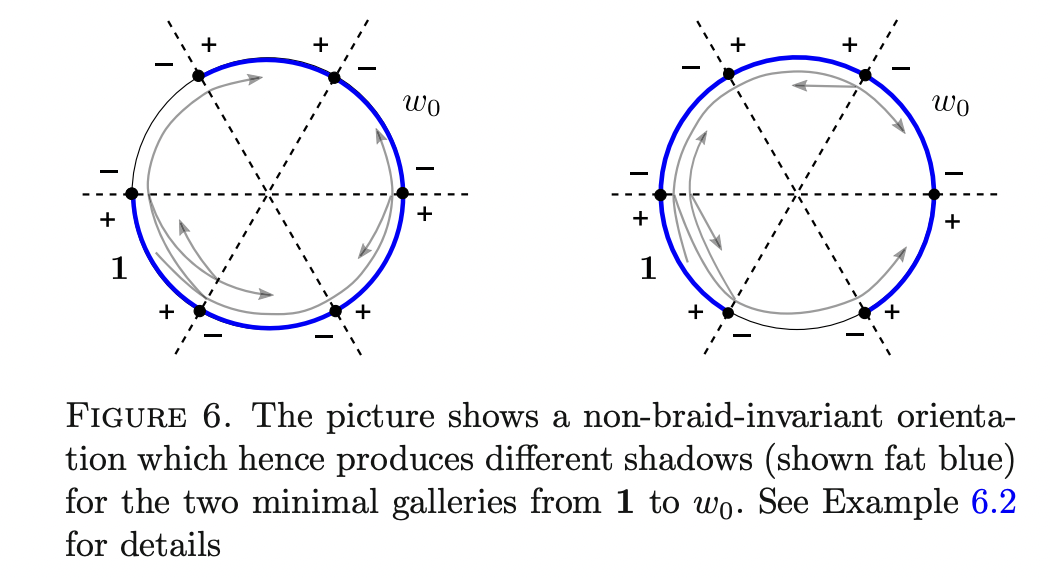
\includegraphics[scale=0.6]{Screenshot 2023-02-08 at 10.39.18.png}\\
\end{center}
\begin{definition}
    Let $x=s_1\hdots s_n$ be a reduced expression for $x\in W$. Let $y\in W$. We say that $y\leq x$ if there exists a reduced expression for $y$ of the form $s_{i_1}\hdots s_{i_k}$ with $1\leq i_1\leq\hdots \leq i_j\leq n$. This ordering is called the \ix{Bruhat order}.
\end{definition}

\begin{proposition}
    Consider the trivial positive orientation $\phi_+$, and the alcove orientation $\phi_1$ towards 1. For $x,y\in W$, $x\geq y$ if and only if $x\stackrel{\phi_+}{\rightharpoonup} y$, if and only if $x\stackrel{\phi_1}{\rightharpoonup} y$.
\end{proposition}

Now this proposition is telling us that actually both the trivial positive orientation and the alcove orientation towards 1 are not interesting orientations to study in terms of the shadow. 

\begin{center}
    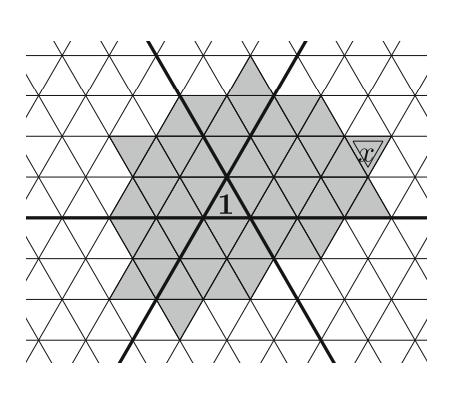
\includegraphics[scale=0.6]{Screenshot 2023-03-07 133912.png}\\
\end{center}


\begin{example}
    The picture above shows the shadow for an alcove of a Coxeter complex of type $\tilde{A}_2$, with respect to the trivial positive orientation. By the proposition above, this is also the shadow with respect to the alcove orientation towards 1. Furthermore, the alcoves in this shadow are all the elements $y$ of the Coxeter group such that $y\leq x$ with respect to the Bruhat ordering, and so it is the Bruhat interval $[1,x]$. 
\end{example}

\subsection{Retractions and shadows}\label{retract}
\tr{Section needs a lot of work.}
We will now see the promised link between retractions and shadows. This comes from looking at the preimage of a retraction map of the building onto a Coxeter complex. 

% First let us consider a general folded gallery lying in a Coxeter complex. We want to show that this gallery is the image under retraction of an unfolded gallery in the building.

% First let us consider a vertex which lies in the dominant Weyl chamber. This is the Weyl chamber which contains the alcove 1. Now let us set an orientation on our 

% A proof of the following theorem can be found in \cite[pp.28-29]{WILD}. The proof given is for vertex-to-vertex galleries, but the proof is esentially the same for alcove-to-alcove galleries. 

% \begin{proposition}
    
% \end{proposition}



Let us first consider when we have a finite Coxeter complex and orientation defined by a chamber $c$. Then we claim that any positive folded gallery is the image of a retraction of an unfolded gallery in the building. This retraction is the chamber retraction towards $d$, where $d$ is the opposite chamber from $c$. 


Now let us consider an affine Coxeter complex with a Weyl chamber orientation. Now here a positively folded gallery is again the image of a retraction of an unfolded gallery in the building. This time, we retract with respect to the Weyl chamber which is opposite the Weyl chamber defining the orientation.






\section{Progress on calculating shadows}\label{9}

So now our main question becomes whether we can calculate the shadow of a given gallery. We have seen in the previous section that this answer with the trivial orientation, and Weyl chamber orientation towards 1, is closely linked to the Bruhat order. 

In general, the question can only be partially answered, and only with specific orientations. Here we will see that if you restrict to looking at Weyl chamber orientations, and affine Coxeter complexes, we can form recursive definitions of the shadows of galleries. This is a partial answer to our question, as we would like a closed form expression for calculating the shadow. 

\subsection{Statistics on positive folds}

We now restrict to looking at Weyl chamber orientations over affine Coxeter complexes. This means that we have a complex \sg, with a boundary $\partial$\sg, and that our orientations are induced by a boundary chamber orientation. Here, we can get a partial answer to our main question of calculating the shadow of a given gallery. To do this, we define a $\phi$-valuation map on our set of alcoves. We can then prove a recursive algorithm for calculating the shadow of a gallery.

First, given a gallery, we want to calculate the number of positive folds of this gallery that we can make. A proof of this proposition can be found in \cite{DEL}.

\begin{proposition}
    Consider the largest element $w_0$ in $W_0$. Given an $x\in W$, and a $\phi$-postive (multi)folding $\gamma$ of $\gamma_x$, we have
    \[l_R(xy^{-1})\leq \mid F(\gamma)\mid \leq l(w_0),\]
    where $y:=\tau($ft$(\gamma))$.
\end{proposition}


\begin{definition}
    Let $\mathcal{H}(\Sigma)$ be the set of all walls contained in our Coxeter complex. For an alcove $c$ of \sg, let $\mathcal{H}(c)$ be the subset of $\mathcal{H}(\Sigma)$ which separates $c$ and the fixed identity alcove 1. Now $\mathcal{H}(c)=\mathcal{H}_{\phi}^+(c)\sqcup \mathcal{H}_{\phi}^-(c)$, where $\mathcal{H}_{\phi}^+(c)$ is the subset of $\mathcal{H}(c)$ such that $c$ lies on the positive side of the walls. Similarly, $\mathcal{H}_{\phi}^-(c)$ is the subset of $\mathcal{H}(c)$ such that $c$ lies on the negative side of the walls..
\end{definition}


\begin{definition}
    Let Ch$(\Sigma)$ denote the set of all alcoves in \sg. The $\phi$-valuation map is the map $\textnormal{v}_\phi:\textnormal{Ch}(\Sigma)\longrightarrow\mathbb{Z}$, with
    \[c\mapsto \textnormal{v}_\phi(c):= \mid \mathcal{H}_{\phi}^+(c)\mid -\mid \mathcal{H}_{\phi}^-(c)\mid .\]
\end{definition}

\begin{definition}
    Let $p_\phi : \textnormal{Ch}(\Sigma)\times \mathcal{H}\longrightarrow \{0,1\}$ be the function 
    \[p_\phi(c,H):= \begin{cases}
        1 & \textnormal{if $c$ is on a $\phi$-positive side of $H$,}\\
        0 & \textnormal{otherwise.}
    \end{cases}\]
\end{definition}

We now want to relate this function to our $\phi$-valuation map.

\begin{lemma}
    \[\textnormal{v}_\phi(c)=\sum_{H\in\mathcal{H}(\Sigma)}(p_{\phi}(c,H)-p_\phi(1,H)).\]
\end{lemma}

\begin{proof}
    We are assuming that our orientation $\phi$ is a chamber orientation. So, in particular, this orientation is locally non-trivial and wall consistent. Therefore, every hyperplane $H$ has a positive and negative side. First consider when 1 and $c$ lie on the same side of $H$. Then $H$ is not an element of $\mathcal{H}(c)$. But, in this case, $p_\phi(1,H)=p_\phi(c,H)$ and so this hyperplane does not contribute to the above sum. 
    Now consider when 1 and $c$ lie on opposite sides of $H$. In this case, $H\in \mathcal{H}(c)$. If $c$ lies on the positive side of $H$, then $H\in\mathcal{H}_{\phi}^+(c)$, $p_\phi(c,H)=1$ and $p_\phi(1,H)=0$, and so $H$ contributes $+1$ to the sum above. Similarly, if $c$ lies on the negative side of $H$, then $H\in\mathcal{H}_{\phi}^-(c)$, $p_\phi(c,H)=0$ and $p_\phi(1,H)=1$, and so $H$ contributes $-1$ to the sum above. Therefore, we are just counting the size of $\mathcal{H}_{\phi}^+(c)$ minus the size of $\mathcal{H}_{\phi}^-(c)$, which is exactly $\textnormal{v}_\phi(c)$. 
\end{proof}


% The next lemma comes from the trivial observation that \[\mid \mathcal{H}_{\phi}^+(c)\mid +\mid \mathcal{H}_{\phi}^+(c)\mid \geq \mid \mathcal{H}_{\phi}^+(c)\mid -\mid \mathcal{H}_{\phi}^+(c)\mid .\]
% \begin{lemma}
%     \[l(x)\geq\textnormal{v}_\phi(c_x).\]
% \end{lemma}

% \begin{definition}
%     We call an alcove $c$ \ix{dominant} with respect to $\phi$ if $\textnormal{v}_\phi(c)=l(c).$
% \end{definition}

% The next two lemmas tell us more information about the $\phi$-valuation map. Proofs can be found in \cite{SHA}.

% \begin{lemma}
%     \[l(x)=\max_{a\in W_0}\textnormal{v}_{\tilde{\phi}_a}(c_x).\]
% \end{lemma}


% \begin{lemma}
%     Let $\phi\in$Dir$(W)$, $r\in W$ be a reflection across the hyperplane $H_r$ and $x\in W$. Then v$_\phi(x)>$v$_\phi(rx)$ if and only if $x$ lies in the $\phi$-positive side of $H_r$. 
% \end{lemma}


\subsection{Computation of regular shadows}

We now want to see how we can use this new valuation map to define a recursive definition of a shadow. To do this, we need the next important theorem. A proof of this theorem can be found in \cite[pp.142-143]{SHA}. 

Let Dir$(W)$ represent the set of chambers in the boundary complex $\partial\Sigma$. We call elements of Dir$(W)$ \ix{directions in W}. 

\begin{theorem} \label{alg}
    Let $\phi\in$Dir$(W)$, $x\in W$ and $s\in S$. Then
    \begin{enumerate}[(i)]
        \item If $s$ is in the right descent set $D_R(x)$ of $x$, then we have
        \[\textnormal{Sh}_\phi(x)=\textnormal{Sh}_\phi(xs)\cdot s \cup \{z\in \textnormal{Sh}_\phi(xs):\textnormal{v}_\phi(zs)<\textnormal{v}_\phi(z)\}.\]
        \item If $s$ is in the left descent set $D_R(x)$ of $x$, then we have
        \[\textnormal{Sh}_\phi(x)=\begin{cases}
            s\cdot \textnormal{Sh}_{s\phi}(sx)\cup \textnormal{Sh}_\phi(sx) &if\textnormal{ v}_\phi(s)<0,\\
            s\cdot \textnormal{Sh}_{s\phi}(sx) &if \textnormal{ v}_\phi(s)>0.\\
        \end{cases}\]
    \end{enumerate}
\end{theorem}


%\begin{definition}
   % Given $x\in W$, $a\in W_0$ and $\phi\in$ Dir$(W)$, the \ix{partial shadow in local direction a} is the set 
   % \[\textnormal{Sh}_\phi^a(x):=\{y\in \textnormal{Sh}_\phi(x)\mid \bar{y}=a\},\]
   % where $\bar{y}$ is the image of $y$ under the natural projection to the spherical Weyl group $W_0$. 
%\end{definition}

Now we can use this theorem to show that the next two lemmas both give us recursive definitions for the shadow of a gallery. 

\begin{lemma} (Algorithm L)
    Let $\phi\in\textnormal{Dir}(W)$ and $x\in W$. Let $w=s_1\hdots s_n$ be a reduced word for $x$. Let $A_0=\{1\}$ and let
    \[A_i:=A_{i-1}\cdot s_i\cup \{z\in A_{i-1}\mid v_\phi(zs)<v_\phi(z)\}.\]
    Then $A_n=\textnormal{Sh}_\phi(x)$. 
\end{lemma}

\begin{proof}
    Using theorem \ref{alg}, we can show by induction that $A_i=$Sh$_\phi(s_1\hdots s_i)$ for $i=0,\hdots ,n$. Firstly, for $i=0$ it is trivial, as Sh$(1)=\{1\}$. Then assume that $A_i=$Sh$_\phi(s_1\hdots s_i)$ for $i<j$. By part (i) of the theorem,\[\begin{aligned}
    \textnormal{Sh}(s_1\hdots s_j)& = \textnormal{Sh}(s_1\hdots s_js_j)\cdot s_j \cup \{z\in \textnormal{Sh}(s_1\hdots s_js_j): \textnormal{v}_\phi(zs)<\textnormal{v}_\phi(z)\}\\
        & = \textnormal{Sh}(s_1\hdots s_{j-1})\cdot s_j \cup \{z\in \textnormal{Sh}(s_1\hdots s_{j-1}): \textnormal{v}_\phi(zs)<\textnormal{v}_\phi(z)\}\\
        & = A_{j-1}\cdot s_j \cup \{z\in A_{j-1}: \textnormal{v}_\phi(zs)<\textnormal{v}_\phi(z)\}\\
        & = A_j.
    \end{aligned}\]
\end{proof}

\begin{lemma} (Algorithm R)
    Let $\phi\in$ Dir$(W)$ and $x\in W$, with $s_n\hdots s_1$ a reduced expression for $x$. Let $B_0^\phi:=\{1\}$ and define
    \[B_i^\phi = \begin{cases}
        s_iB_{i-1}^{s_i\phi}\cup B_{i-1}^\phi & \textnormal{if v}_\phi(s_i)<0,\\
        s_iB_{i-1}^{s_i\phi} & \textnormal{if v}_\phi(s_i)>0.
    \end{cases}\]
    Then $B^\phi_n=$Sh$_\phi(x)$ for all $\phi\in$ Dir$(W)$. 
\end{lemma}

\begin{proof}
    Again, we can use theorem \ref{alg} to prove by induction that $B^\phi_i=$Sh$_\phi(s_i\hdots s_1)$ for all $i=0,\hdots ,n$. For $i=0$ it is trivial, as Sh$_\phi(1)=\{1\}$. Now assume that $B^\phi_i=$Sh$_\phi(s_i\hdots s_1)$ for all $i<j$. By part (ii) of the theorem, if $v(s_j)<0$, then
    \[\begin{aligned}
        Sh_\phi(s_j\hdots s_1)&=s_j\cdot \textnormal{Sh}_{s_j\phi}(s_js_j\hdots s_1)\cup \textnormal{Sh}_\phi(s_js_j\hdots s_1)\\
                        &=  s_j\cdot \textnormal{Sh}_{s_j\phi}(s_{j-1}\hdots s_1)\cup \textnormal{Sh}_\phi(s_{j-1}\hdots s_1)\\
                        &= s_j\cdot B^{s_j\phi}_{j-1}\cup B^{\phi}_{j-1}\\
                        &= B^\phi_j. 
    \end{aligned}\]
    Similarly, if $v(s_j)>0$, then
    \[\begin{aligned}
        Sh_\phi(s_j\hdots s_1)& = s_j\cdot \textnormal{Sh}_{s_j\phi}(s_js_j\hdots s_1)\\
                        & = s_j\cdot \textnormal{Sh}_{s_j\phi}(s_{j-1}\hdots s_1)\\
                        & = s_j \cdot B^{s_j\phi}_{j-1}\\
                        & = B^{\phi}_{j}. 
    \end{aligned}\]
\end{proof}


\section{Conclusion}

In this paper we have defined buildings and Coxeter complexes, and defined galleries in Coxeter complexes. We have looked at different orientations we can place on our given Coxeter complex, and how we can define positive foldings of galleries with respect to orientations. This leads to a natural question of calculating the shadow of a gallery. We have seen some progress made so far in answering this question, but we are yet to find a non-recursive answer to calculating the shadow of a gallery. Our next step is to try to answer this question for specific orientations. We have seen in this paper that the answer, for the trivial orientation and the orientation at inifinity in the direction of 1, is completely related to the Bruhat ordering on our Coxeter group. It is reasonable to propose that, with other orientations, there is a link to Bruhat ordering, or possibly some other type of ordering on our Coxeter group elements. 

\newpage
\bibliographystyle{abbrv}
%\nocite{*}
\bibliography{references}

\end{document}